\documentclass[12pt, a4paper,oneside, openany]{book}
%fuente12pt,tamaño carta,una cara,quitar hojas en blanco,tipo libro
\usepackage[utf8]{inputenc} %fuente Unicode
%\usepackage[margin=-0cm]{geometry} %margen
\usepackage{graphicx} %uso de imagenes
\usepackage{multicol} %uso de multicolumnas
\usepackage{multirow} %multi celdas
\usepackage{lastpage} %n.total de paginas
\usepackage{colortbl} %columnas de color
\usepackage{tikz, tikz-3dplot} %figuras
\usepackage{tkz-euclide}
\usepackage{adjustbox} %manejo de margenes
\usepackage[spanish]{babel} %lenguaje español
\usepackage[document]{ragged2e} %alineacion
\usepackage[T1]{fontenc} %codificacion fuente
\usepackage{enumerate} %viñeta numeros
\usepackage{palatino} %fuente
\usepackage[colorlinks,linkcolor=myblue,citecolor=mygreen]{hyperref} %link personalizado
%-----------------------------------------------------------------
\definecolor{myblue}{HTML}{2D74B5} %color de titulos y subtitulos
%-----------------------------------------------------------------
\graphicspath{ {img/} } %localizacion de carpeta con imagenes
\renewcommand{\baselinestretch}{1.2} %espacio entre parrafos

%\AtBeginDocument{\AtBeginShipoutNext{\AtBeginShipoutDiscard}}
%elimina paginas adicionales que se agregan con el uso de hyperref
\usepackage{multirow} %multi celdas en tablas
\usepackage{longtable} %tablas multipagina
\usepackage{caption} %ajuste de tablas, figuras
\usepackage{color} %colores de texto
\usepackage{wrapfig} %rodear imagenes
\usepackage{booktabs, multirow} %bordes y rangos
\usepackage{titlesec} %titulos personalizados
\usepackage{eso-pic,picture} %imagenes con texto
\usepackage{nomencl} %simbolos de nomenclatura
\usepackage{lipsum} %crea texto default
\makenomenclature %tamaño nomenclatura
%\usepackage{showframe} %muestra el margen de las pg
%-----------------------------------------------------------------
%codigo del borde
\AddToShipoutPicture{%
\setlength\fboxsep{1pt}%
\put(24pt,24pt){\framebox(19.3066cm,28.0066cm)[lb]{}}%
}

%margenes
\usepackage{geometry}
\newgeometry{
        top=0.001in,
        bottom=3.2in,
        outer=0.55in,  %izquierda
        inner=0.55in, %derecha
        }
%-----------------------------------------------------------------
\usepackage{fancyhdr}%uso de encabezado y pie personalizado
\pagestyle{fancy}

\setlength{\headheight}{160pt}%ubicacion de caja de encabezado

\titlespacing{\chapter}{0pt}{-42pt}{0.5cm}%config capitulos, espacio de chapter
\titleformat{\chapter}[display]
{\sffamily\color{myblue}} {
    {\normalfont\color{myblue}\Large}
        \hspace{0pt}
            {\setlength\fboxsep{0pt}
                \colorbox{myblue}{
                }
            }
    }
{0 pt}
{\titlerule[0pt]\LARGE\sffamily}

%%%%%%%%%%%%%%%%%%%%%%%%%%%%%%%%%%%%%%%%%%%%%%%%%%%%%%%%%%%%%%%%%%%%%%%
\fancyhf{}%Declaración de encabezado
\pagestyle{fancy}
\fancypagestyle{plain}{}%encabezado general

\begin{document}%inicio de documento

\lhead{

\begin{minipage}{0.1\textwidth}
\scalebox{1}[1.2]{
\begin{tabular}{|m{2cm}|m{10.8cm}|m{1.0cm}|m{1.0cm}|m{1.0cm}| }

\hline

\multirow{3}{2cm}{\centering
\includegraphics[width=0.88\textwidth]{tjacdmx_logo.png}}
& \footnotesize\centering\bf\sffamily{TRIBUNAL DE JUSTICIA ADMINISTRATIVA DE TABASCO}
& \footnotesize\bf\sffamily{Día}
& \footnotesize\bf\sffamily{Mes}
&\footnotesize\bf\sffamily{Año}
\\ \cline{2-5}

& \centering\bf\footnotesize\sffamily{DIRECCIÓN GENERAL DE ADMINISTRACIÓN}
& \footnotesize\bf\sffamily{27}
& \footnotesize\bf\sffamily{02}
& \footnotesize\bf\sffamily{2023}
\\ \cline{2-5}

& \centering\bf\footnotesize\sffamily{DIRECCIÓN DE INFORMÁTICA}
& \multicolumn{3}{ |c| }{\bf\footnotesize\sffamily{Versión: 001 }}
\\ \cline{2-5}

&
\centering\bf\footnotesize\sffamily{MANUAL DE USUARIO}
& \multicolumn{3}{ |c| } {\bf\footnotesize\sffamily{Página \thepage~de\ \pageref{LastPage}}}
\\ \hline

\end{tabular}}
\end{minipage}

}
%-----------------------------------------------------------------

\centerline{
\includegraphics[width=0.8\textwidth]{tjacdmx_logo.png}}%imagen de logo en portada
%titulo de portada

\vspace{1cm}%espacio
%-----------------------------------------------------------------
\begin{flushright}%alineación a la derecha

\newcommand{\ProjectTitle}

\vspace{0cm}
%titulo en portada
{\color{myblue}{\sffamily\large\bf\sffamily
ACTUARIA V3.0 \\
GENERACIÓN DE CÉDULAS  V2.0.0\\
\vspace{0.3cm}
MANUAL DE USUARIO\\
\vspace{0.2cm}
DIRECCIÓN DE INFORMÁTICA}
}

\end{flushright}
%-----------------------------------------------------------------
%pie de todas las paginas
\cfoot[]{
{\tiny
\scalebox{1}[1.2]{%tamaño de celdas
\centering\begin{tabular}{|m{4cm}|m{4.0cm}|m{4.0cm}|m{4.0cm}| }

\hline

\centering\sffamily IDENTIFICACIÓN
& \centering\sffamily ELABORÓ
&  \centering\sffamily REVISÓ
& AUTORIZÓ
\\
\hline

\centering\sffamily TJACDMX DI MANUAL USUARIO
&  \centering\sffamily Dirección de Informática
&  \centering\sffamily Dirección de Informática
&  Comité Técnico Interno de Administración de Documentos del
TJACDMX en su sesión...
\\
\hline
\end{tabular}}

}}
%-----------------------------------------------------------------


\renewcommand{\headrulewidth}{0pt}%sin linea por default
\begin{quote}%alineacion de texto

\tableofcontents

\chapter{\large{Objetivo}}\label{chap:objetivo}
Con la finalidad de ofrecer a los servidores públicos del Tribunal de Justicia Administrativa de Tabasco
una herramienta que facilite la operación de los apartados que integran el módulo
de «Actuaría v 3.0», se elaboró el presente Manual.

\chapter{\large{¿Cómo ingresar a Actuaría v3.0?}}\label{chap:ingreso}

1.Ingresaremos al Sistema con el siguiente link:

\begin{center}
\href{https://sidj.tjacdmx.gob.mx}{https://sidj.tjacdmx.gob.mx}
\end{center}

2.Nos ubicaremos en el menú y daremos clic en  {\bf{
<<Actuaria v3.0>> }}

\begin{center}
    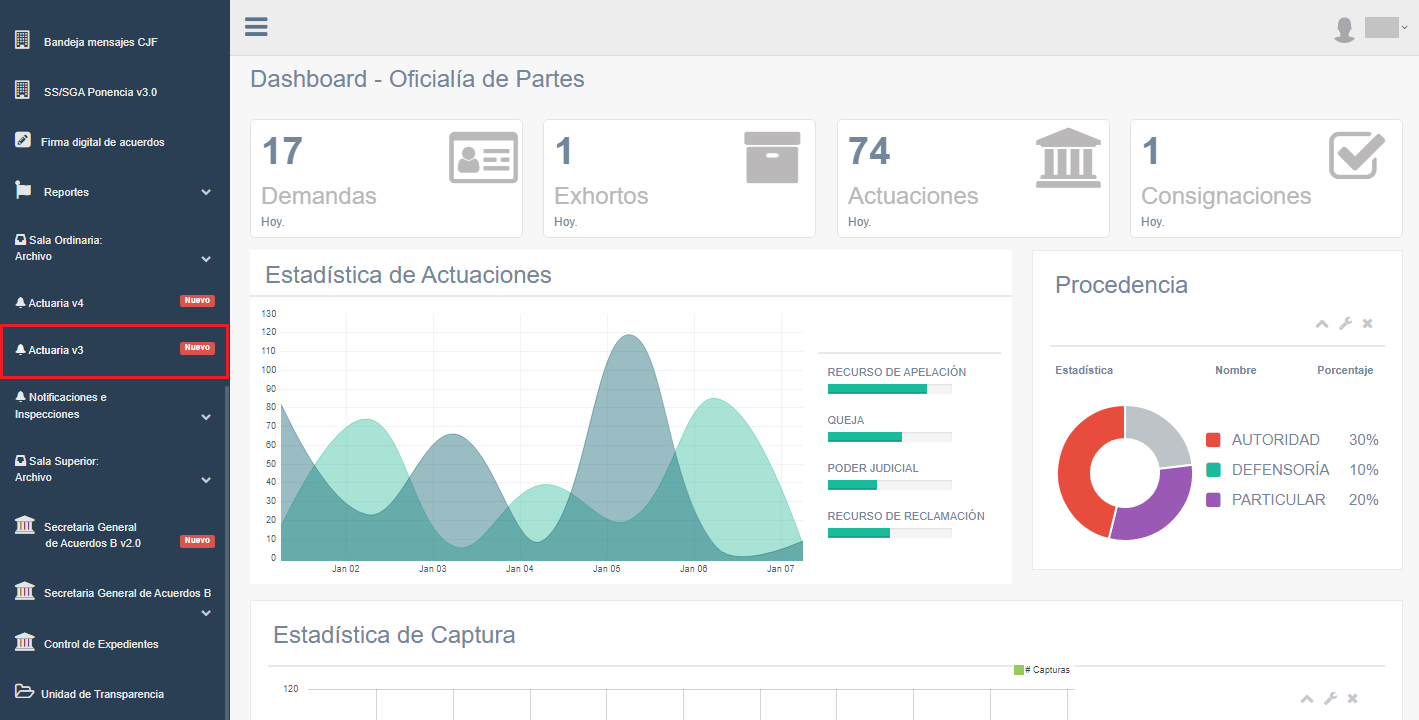
\includegraphics[width=0.88\columnwidth]{inicioAc.png}
\end{center}

\chapter{\large{Generación de cédulas v2.0.0}}\label{chap:cedulas}
{\Huge{\color{myblue} \section{¿Cómo generar una cédula?}\label{sec:12}}}

Daremos clic en la opción {\bf{ <<Generación de cédulas v2.0.0>>  }}

\begin{center}
    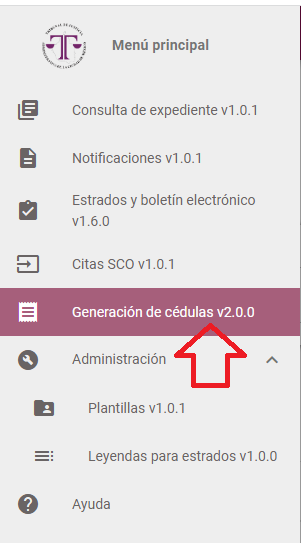
\includegraphics[width=0.20\columnwidth]{cedulas.png}
\end{center}

Para generar una cédula existe 3 opciones:

 \begin{enumerate}[(1)] 
        \item Escaneando el folio del acuerdo.
	\item Ingresando el folio manualmente.
	\item Subiendo archivo de excel con los folios de acuerdo.
\end{enumerate}


\begin{center}
    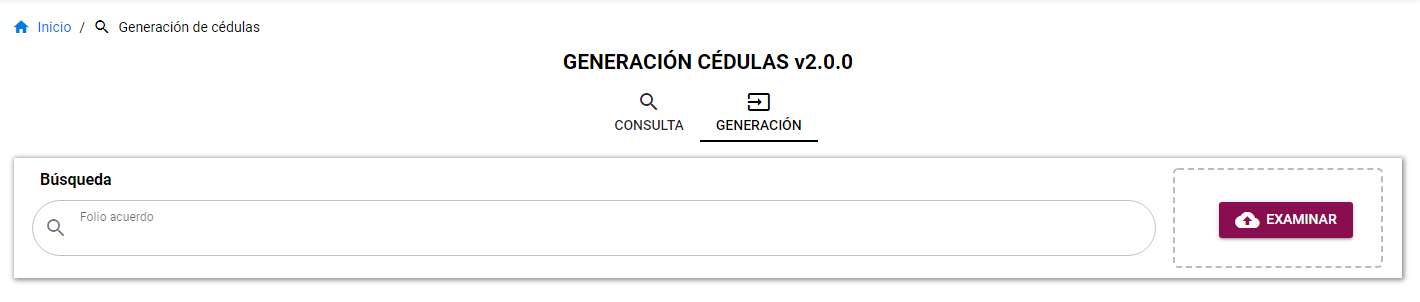
\includegraphics[width=0.90\columnwidth]{exam.png}
\end{center}

Después de escanear o ingresar manualmente el folio nos mostrara la siguiente pantalla, 
para seleccionar las notificaciones para acuerdo.

\begin{center}
    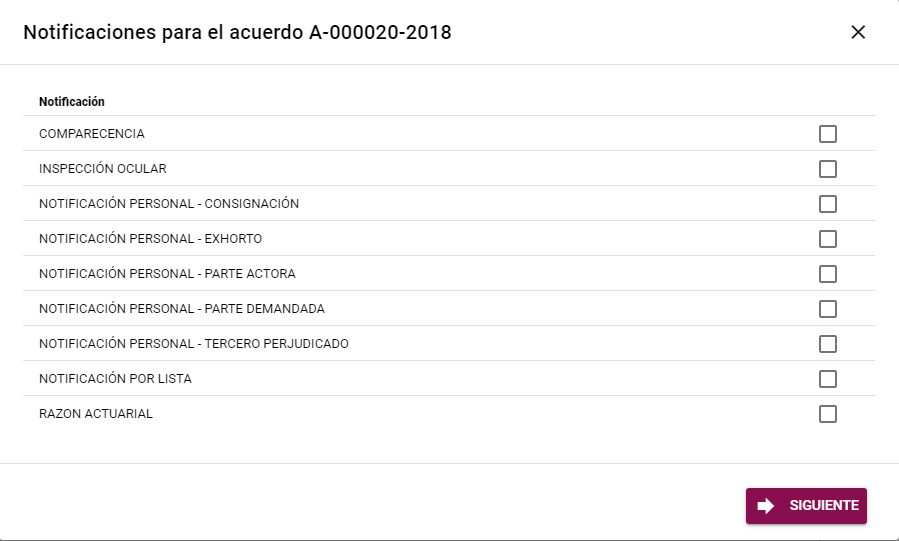
\includegraphics[width=0.90\columnwidth]{noti5.png}
\end{center}

Se podrá seleccionar más de una notificación por acuerdo. Una vez seleccionado la(s)
notificación(es), da clic en el botón {{\bf«SIGUIENTE»}}, mostrara el siguiente formulario con los siguientes
datos:

\begin{center}
    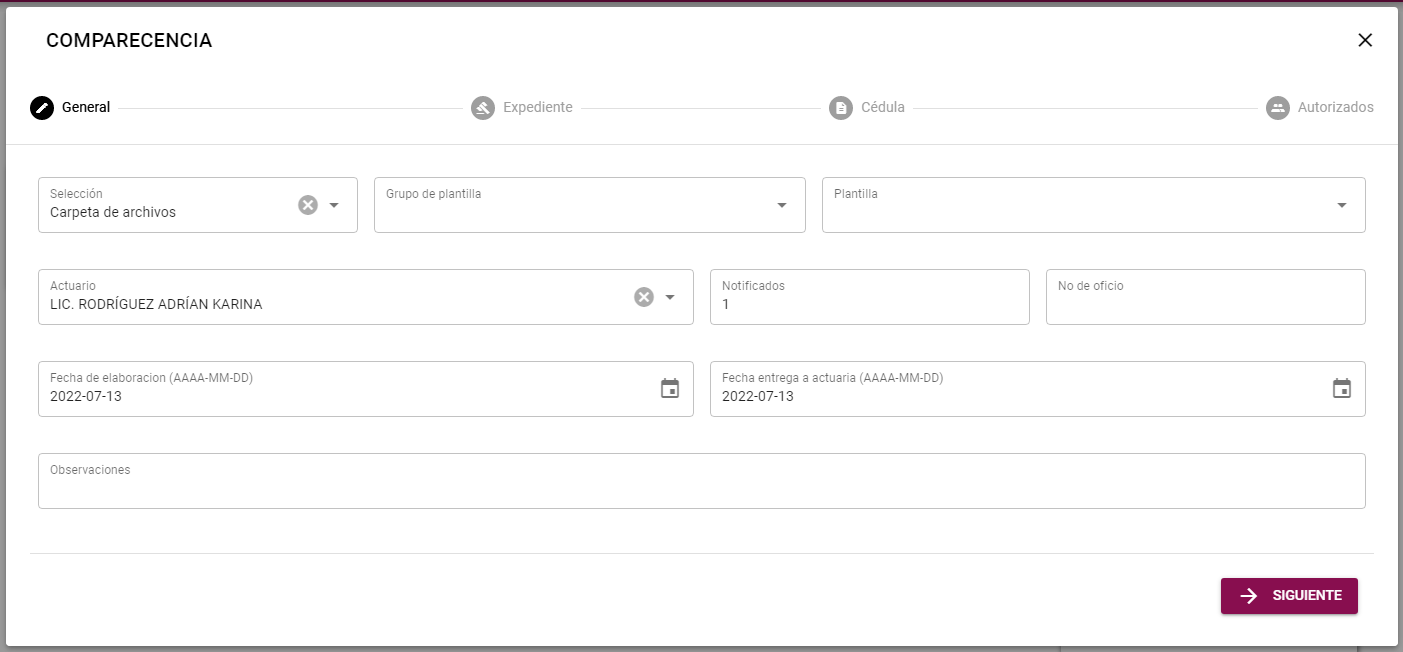
\includegraphics[width=0.90\columnwidth]{comparecencia.png}
\end{center}

\begin{itemize}
    \item Selección
    \item  Grupo de plantilla
    \item  Plantilla
    \item  Actuario
    \item  Notificados
    \item  No de oficio
    \item  Fecha entrega a actuaria
    \item  Fecha de elaboración
    \item Observaciones
\end{itemize}

En caso de no contar con una plantilla registrada en el sistema, se puede subir una plantilla
temporal.\\

Primero tienes que seleccionar:
{\bf{
<<Subir archivo>>}}y dar clic en subir archivo.\\

\begin{center}
    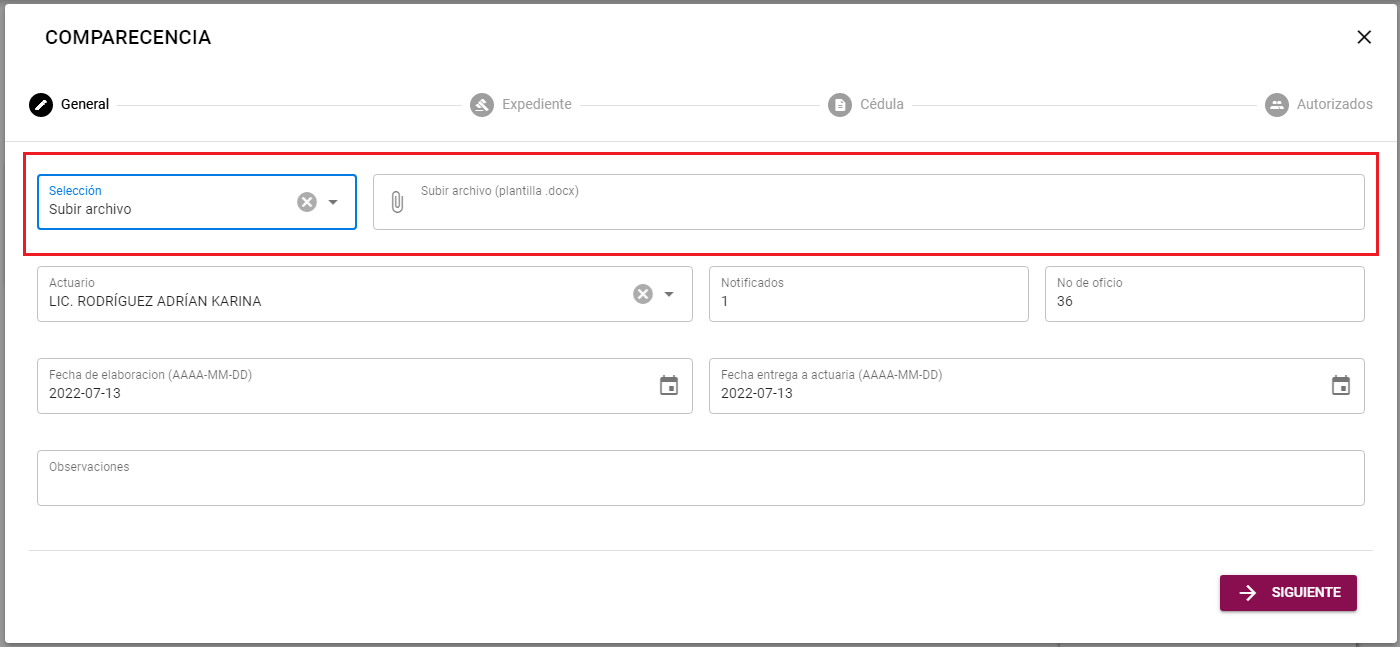
\includegraphics[width=0.90\columnwidth]{comparecencia3.png}
\end{center}

Automáticamente se abrirá una ventana donde seleccionaras tu plantilla desde tus documentos.

\begin{center}
    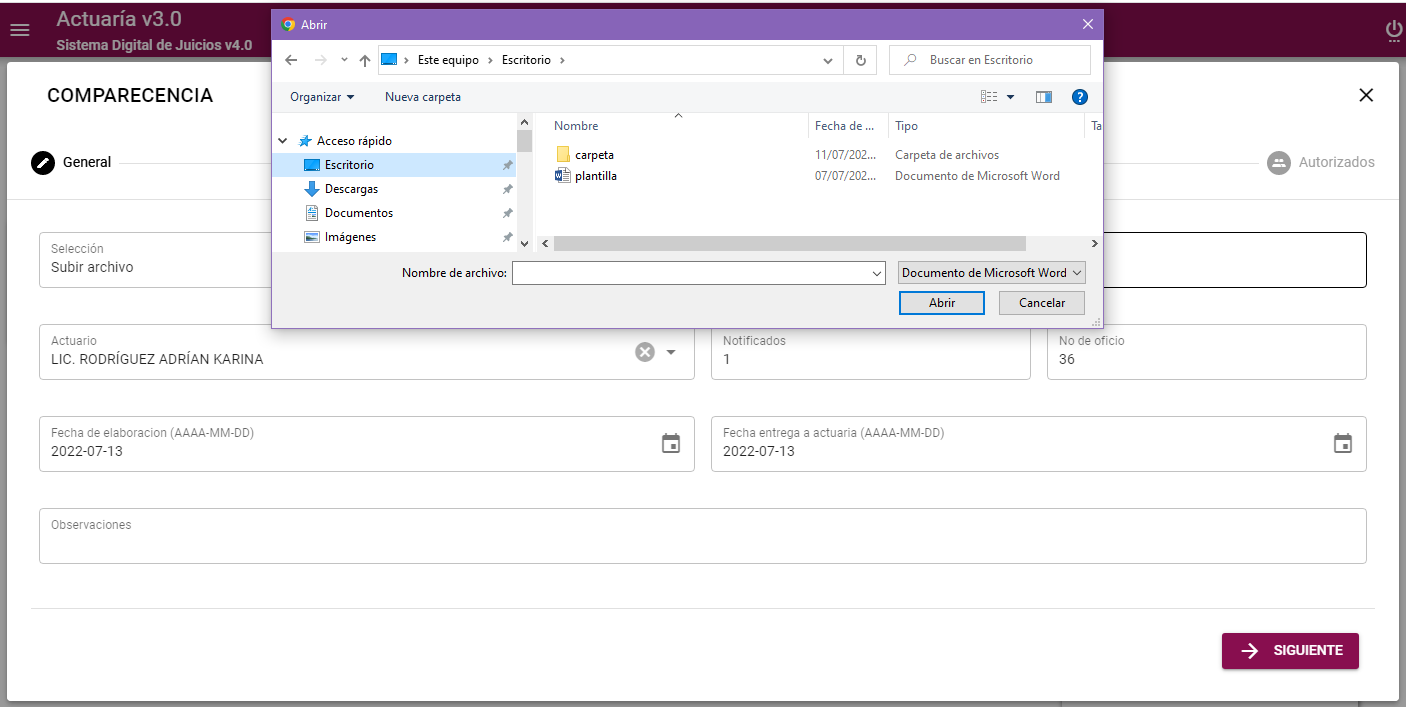
\includegraphics[width=0.90\columnwidth]{comparecencia4.png}
\end{center}

Después de ingresar los datos daremos clic en el botón.
{\bf{<<SIGUIENTE>>}}
Ahora ingresaremos los siguientes datos:

 \begin{itemize}
    \item Teléfono
	\item Correo electrónico
	\item Domicilio para recibir notificaciones (*)
 \end{itemize}


\begin{center}
    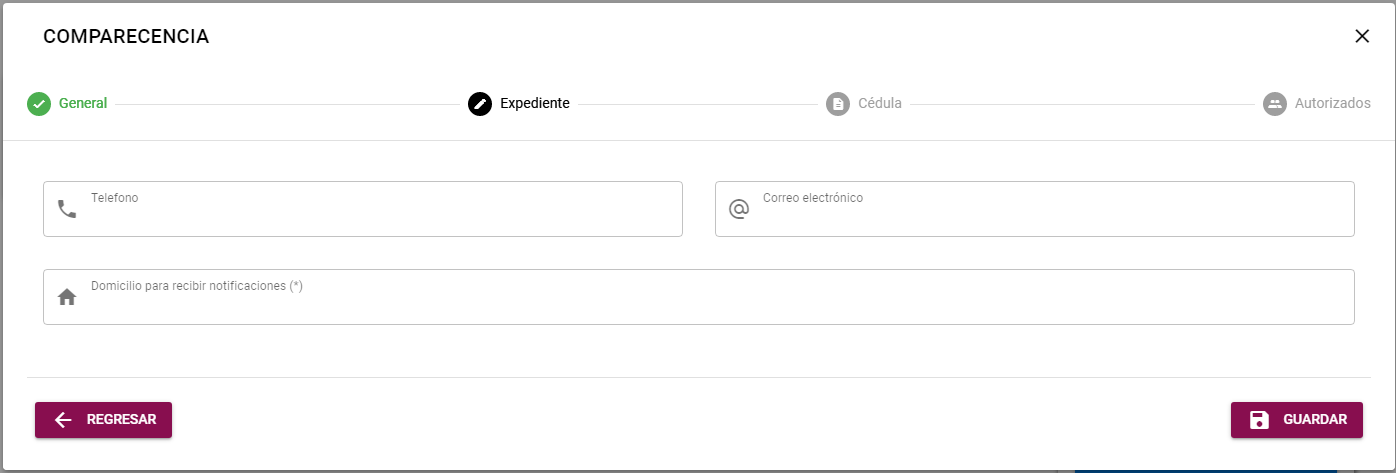
\includegraphics[width=0.90\columnwidth]{comparecencia2.png}
\end{center}

Daremos clic en {\bf{
<<GUARDAR>>}}

{\Huge{\color{myblue} \section{¿Cómo generar cédula desde un archivo de Excel?}\label{sec:13}}}

Para usar la opción de  Archivo de Excel es requerido que el archivo cuente con las siguientes condiciones:\\
Para  {{\bf<<NOTIFICACIÓN PERSONAL>>}} el archivo debe tener los siguientes títulos al inicio del Excel en la fila 1:

\begin{multicols}{2} %multicolumnas
\begin{itemize}
    \item  no\_folio\_acuerdo
    \item  oficio
    \item  notificados
    \item  actores
    \item  tipo\_notificación
    \item  terceros
    \item  tipo\_acuerdo
    \item  fecha\_elaboración\_acuerdo
    \item  fecha\_elaboración\_cédula
    \item  fecha\_entrega\_actuaria
    \item  folio
    \item  teléfonos\_expediente
    \item  lic
    \item  anexo
    \item  domicilio\_notificaciones
    \item  autorizados
    \item  email\_expediente
    \item  autoridades
\end{itemize}
\end{multicols}

Todos los títulos en {{\bf minúsculas y separando palabras con guión bajo \_}}.

Ejemplo:
\begin{center}
    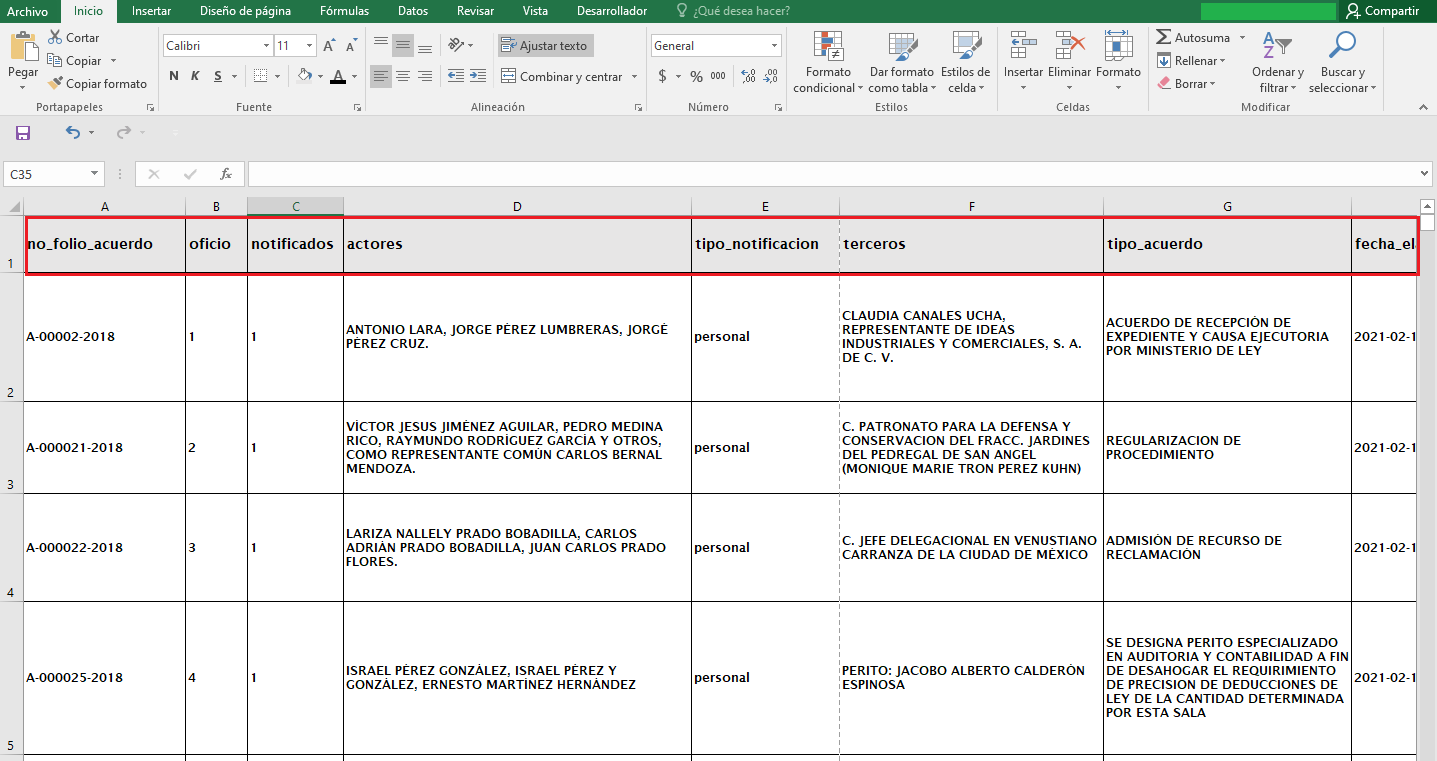
\includegraphics[width=0.80\columnwidth]{EJEM.png}
\end{center}

Los campos de:

\begin{itemize}
    \item  actores
    \item  autorizados
\end{itemize}


Se requiere que sean {{\bf separados por coma, cada nombre}} ejemplo de {{\bf actores}}:\\

\begin{center}
    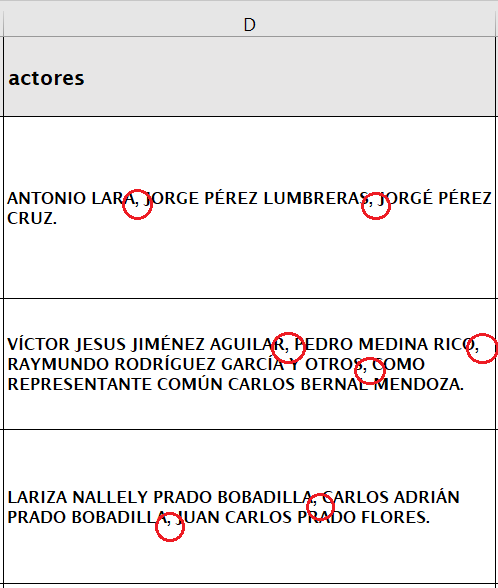
\includegraphics[width=0.50\columnwidth]{act.png}
\end{center}

ejemplo de {{\bf autorizados}}:\\

\begin{center}
    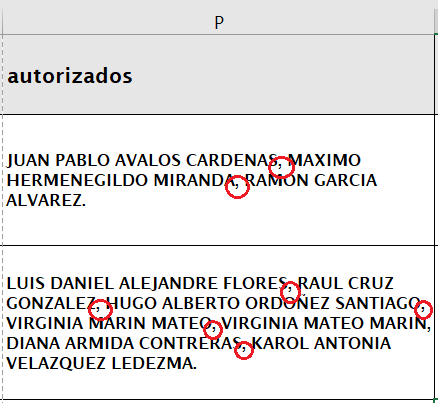
\includegraphics[width=0.50\columnwidth]{aut.png}
\end{center}

Los campos de

\begin{itemize}
    \item  fecha\_elaboracion\_acuerdo
    \item  fecha\_elaboracion\_cedula
    \item  fecha\_entrega\_actuaria
\end{itemize}


Tienen que tener el formato de {{\bf AÑO-MES-DÍA  }}
Ejemplo:

\begin{center}
    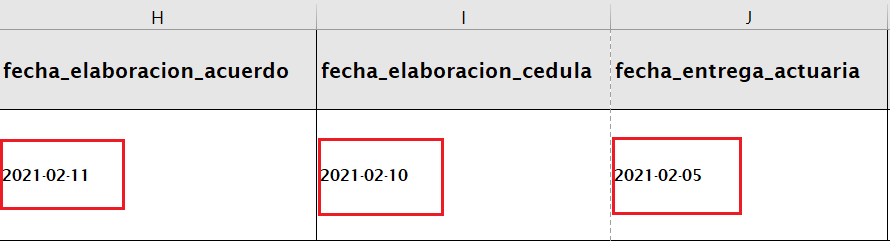
\includegraphics[width=0.60\columnwidth]{formato.png}
\end{center}

Teniendo nuestro archivo con el formato correcto, daremos clic en el botón  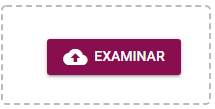
\includegraphics[width=0.15\columnwidth]{examinar.png}
automáticamente se nos abrirá una ventana donde seleccionaremos nuestro archivo de Excel y daremos clic en el botón {\bf{ <<Abrir>>}}

\begin{center}
    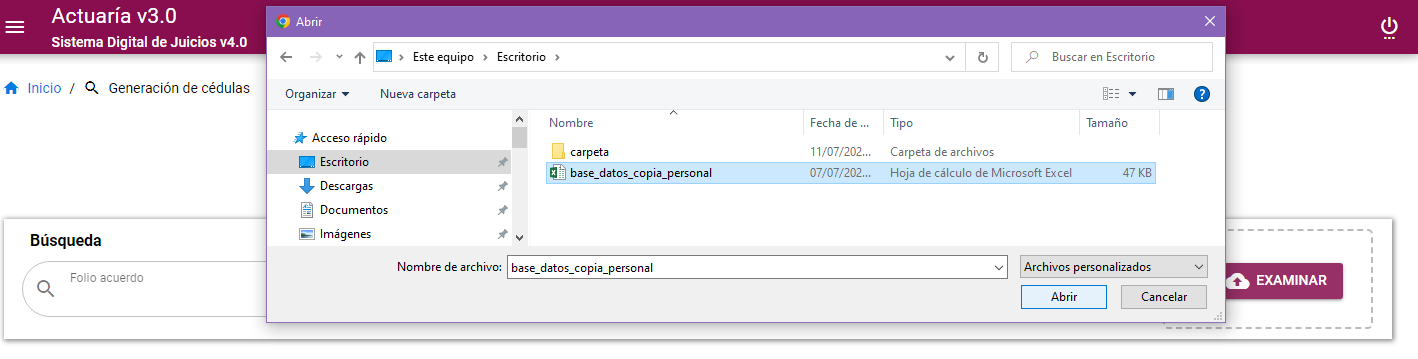
\includegraphics[width=0.90\columnwidth]{exam2.png}
\end{center}

El sistema mostrará la siguiente pantalla:
\begin{center}
    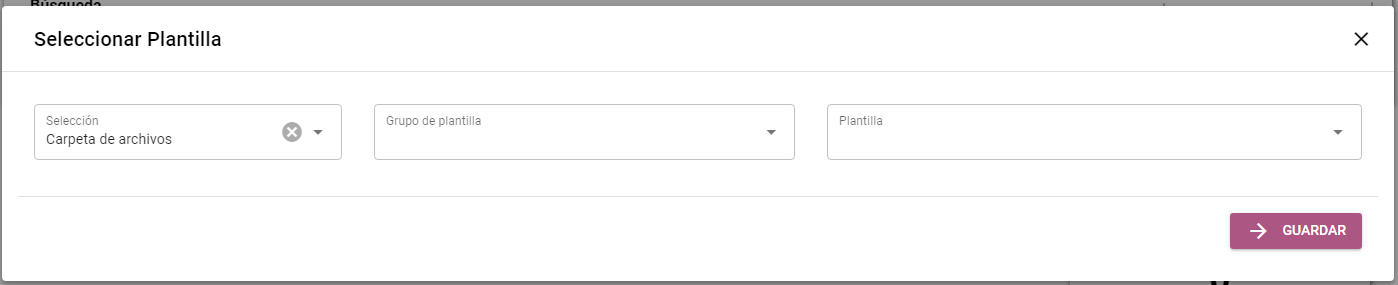
\includegraphics[width=0.90\columnwidth]{select.png}
\end{center}

Seleccionaremos :
\begin{itemize}
    \item  Carpeta
    \item  Grupo de plantilla
    \item  Plantilla
\end{itemize}

En caso de no contar con una plantilla registrada en el sistema, se puede subir una plantilla
temporal.\\
Primero tienes que seleccionar: Subir archivo y dar clic en subir archivo para que abra la ventana para seleccionar archivo.

\begin{center}
    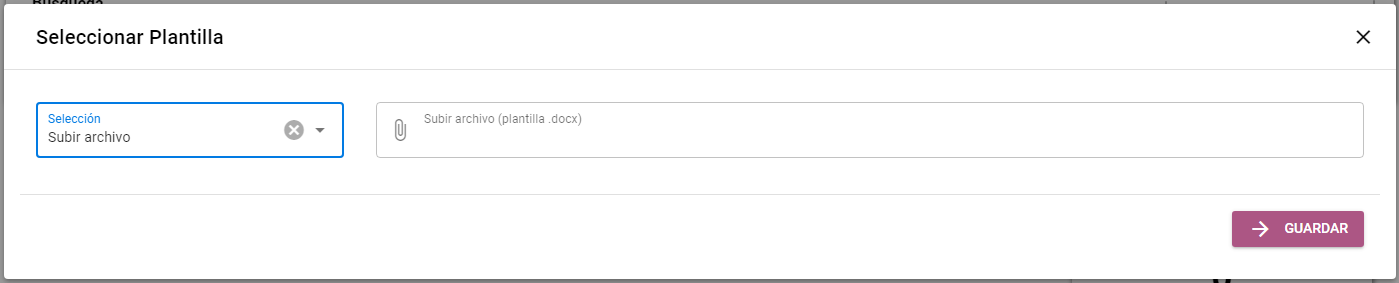
\includegraphics[width=0.90\columnwidth]{select2.png}
\end{center}

Después de ingresar los datos daremos clic en el botón
{\bf{
<<SIGUIENTE>>}}\\
Nos aparecerá una alerta con el estatus de los acuerdos ingresados por el excel, en este caso de ejemplo 
podemos ver que dice que se cargaron 0 acuerdos correctamente, por lo tanto hay 5 acuerdos con errores y 
nos menciona que podemos ver los errores dando clic en el icono     

\includegraphics[width=0.05\columnwidth]{icob.png}

\begin{center}
    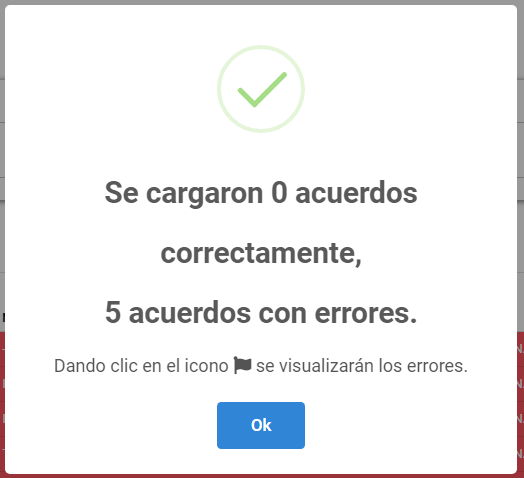
\includegraphics[width=0.50\columnwidth]{alert2.png}
\end{center}

En el caso de tener errores los acuerdos se marcaran en rojo y recorriendo la barra de abajo nos aparecerá el icono de bandera
como en el siguiente ejemplo:

\begin{center}
    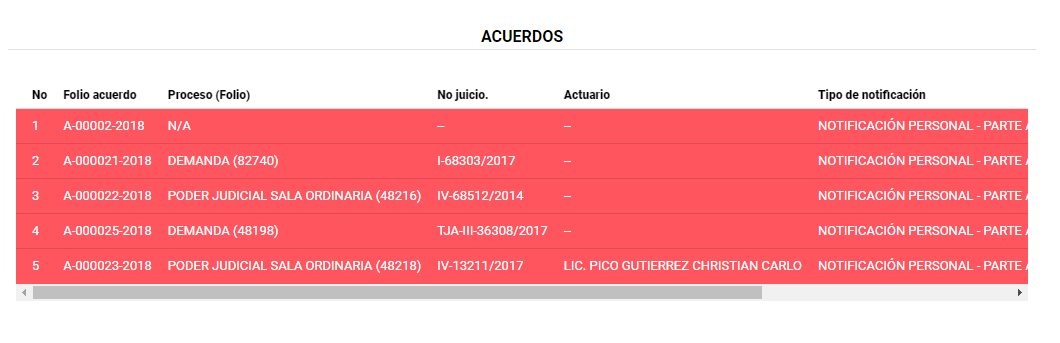
\includegraphics[width=0.90\columnwidth]{bandera.png}
\end{center}

Al recorrer la barra podemos observar el icono de bandera

\begin{center}
    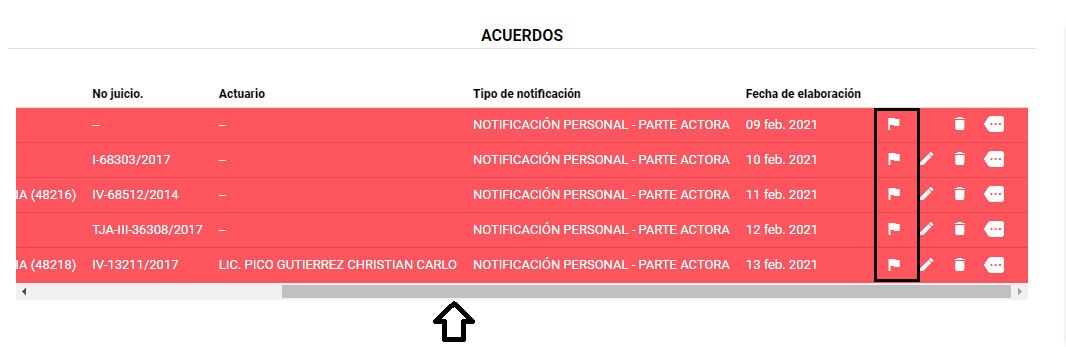
\includegraphics[width=0.90\columnwidth]{bandera2.png}
\end{center}

Al seleccionar el icono podemos ver el error como a continuación.

\begin{center}
    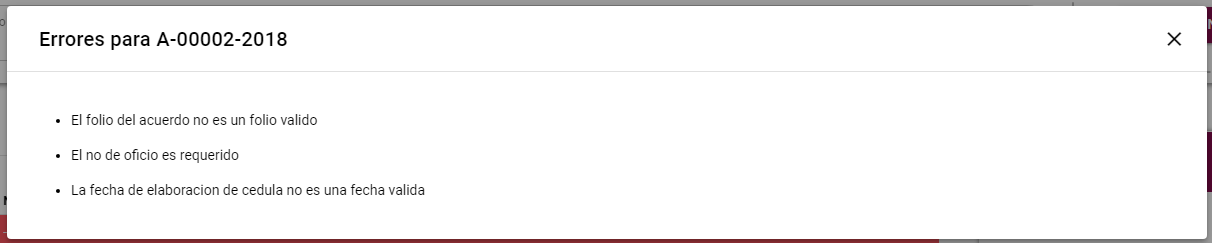
\includegraphics[width=0.90\columnwidth]{errores.png}
\end{center}

Podemos ver que :\\
El folio del acuerdo no es un folio valido\\
El no de oficio es requerido\\
La fecha de elaboración de cédula no es una fecha valida \\

En este caso tenemos dos opciones:
\begin{enumerate}[1.]
    \item Usar las opciones de corrección del sistema.
    \item Borrar y volver a subir el archivo corregido
\end{enumerate}


\vspace{1cm}

{{\bf1. Usar las opciones de corrección del sistema}}\\
Para solucionar los errores del ejemplo.

El sistema nos permite  {{\bf<<Editar el folio de acuerdo>>}}
dando clic en el Folio acuerdo

\begin{center}
    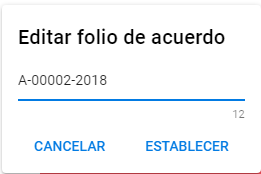
\includegraphics[width=0.40\columnwidth]{edifolio.png}
\end{center}

Después de ingresar el dato correcto daremos clic en {{\bf
<<ESTABLECER>>}} el sistema automáticamente verificará si es correcto o no, en caso de error seguirá marcado con rojo.\\
Ahora utilizando el icono {{\bf<<EDITAR>>}}
podemos agregar el número de oficio y editar la fecha.\\

Daremos clic en el icono  <<Editar>>

\begin{center}
    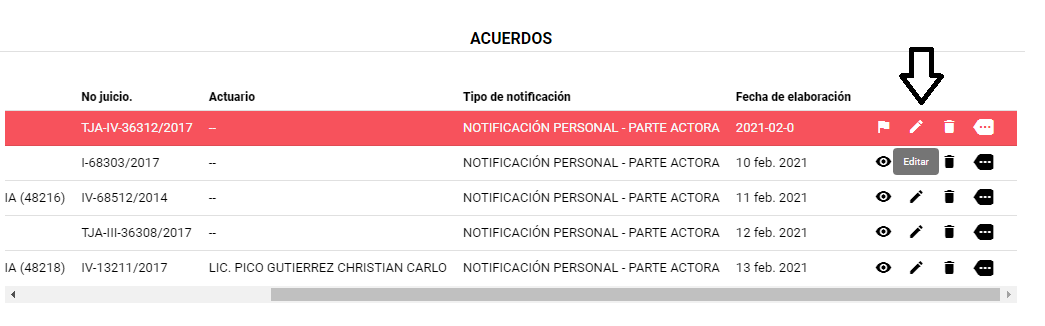
\includegraphics[width=0.90\columnwidth]{editarac.png}
\end{center}

El cual nos abrirá la siguiente ventana:

\begin{center}
    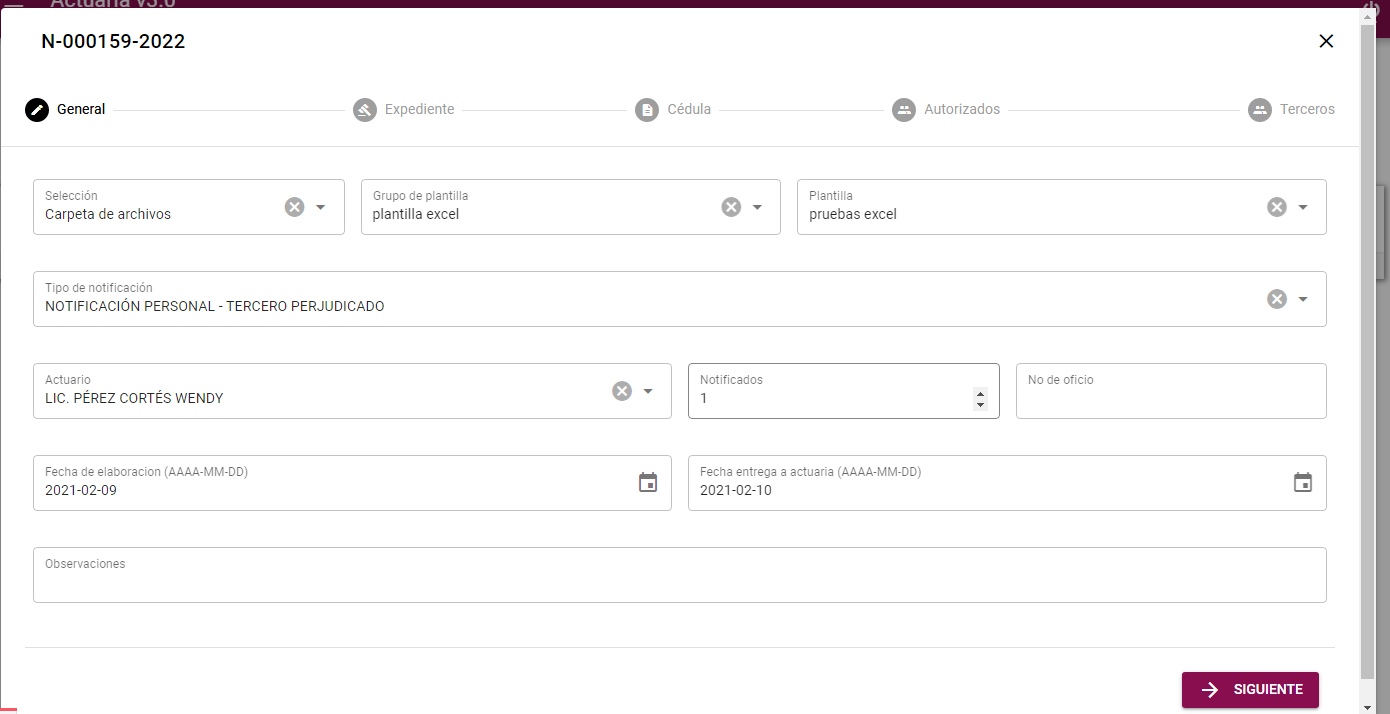
\includegraphics[width=0.90\columnwidth]{editaracuerdo.png}
\end{center}

Nos ubicará en  <<General>> aquí
ingresaremos el número de oficio y corregiremos la fecha de elaboración de célula.\\
Daremos clic en el botón  {{\bf<<SIGUIENTE>>}} nos aparecerá la siguiente ventana:

\begin{center}
    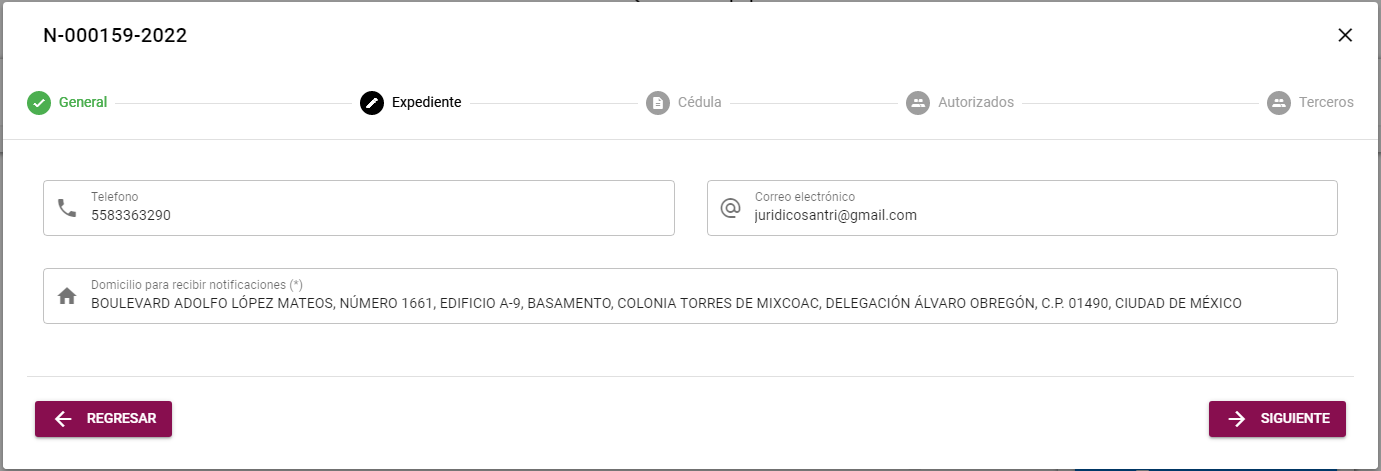
\includegraphics[width=0.90\columnwidth]{editaracuerdo2.png}
\end{center}

Podemos revisar nuestros datos o corregir el deseado y
daremos clic en el botón  {{\bf<<SIGUIENTE>>}} nos aparecerá la siguiente ventana:

\begin{center}
    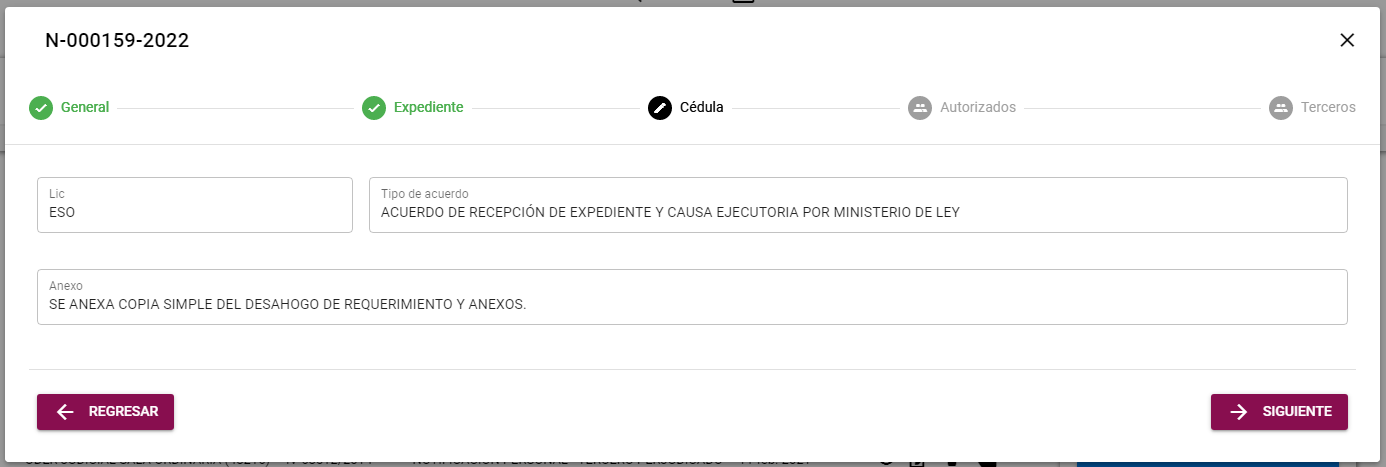
\includegraphics[width=0.90\columnwidth]{editaracuerdo3.png}
\end{center}

De igual forma podemos revisar nuestros datos o corregir el deseado y
daremos clic en el botón  {{\bf<<SIGUIENTE>>}}
nos aparecerá la siguiente ventana:

\begin{center}
    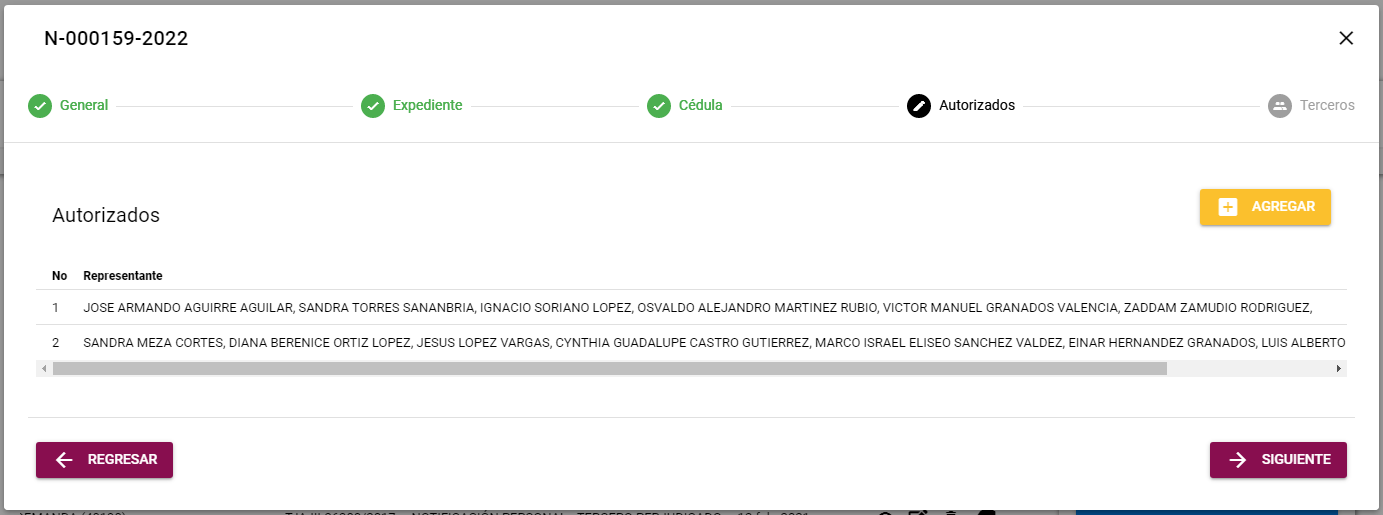
\includegraphics[width=0.90\columnwidth]{editaracuerdo4.png}
\end{center}

daremos clic en el botón  {{\bf<<SIGUIENTE>>}} nos aparecerá la siguiente ventana:

\begin{center}
    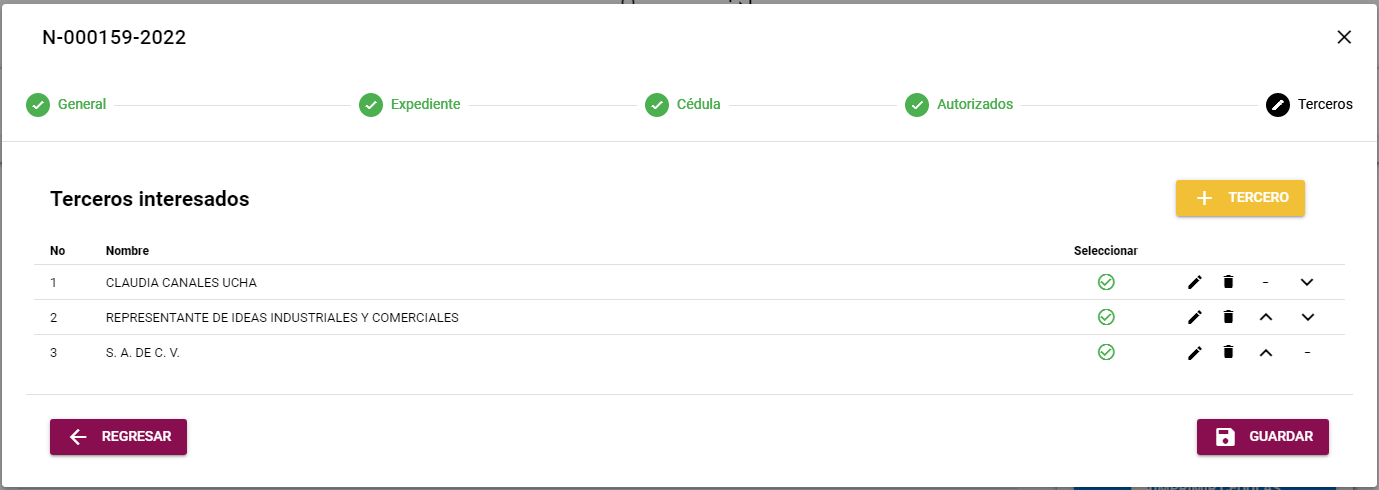
\includegraphics[width=0.90\columnwidth]{editaracuerdo5.png}
\end{center}

Daremos clic en el botón {\bf{<<GUARDAR>>}} si los datos de nuestros acuerdos son correctos
nos aparecerá el siguiente mensaje:

\begin{center}
    
\includegraphics[width=0.30\columnwidth]{cedulaguardada.png}
\end{center}

Seguido de este mensaje.
\begin{center}
    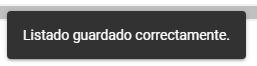
\includegraphics[width=0.33\columnwidth]{listadoguardado.png}
\end{center}

Ahora ya podemos visualizar nuestros acuerdos corregidos.

\begin{center}
    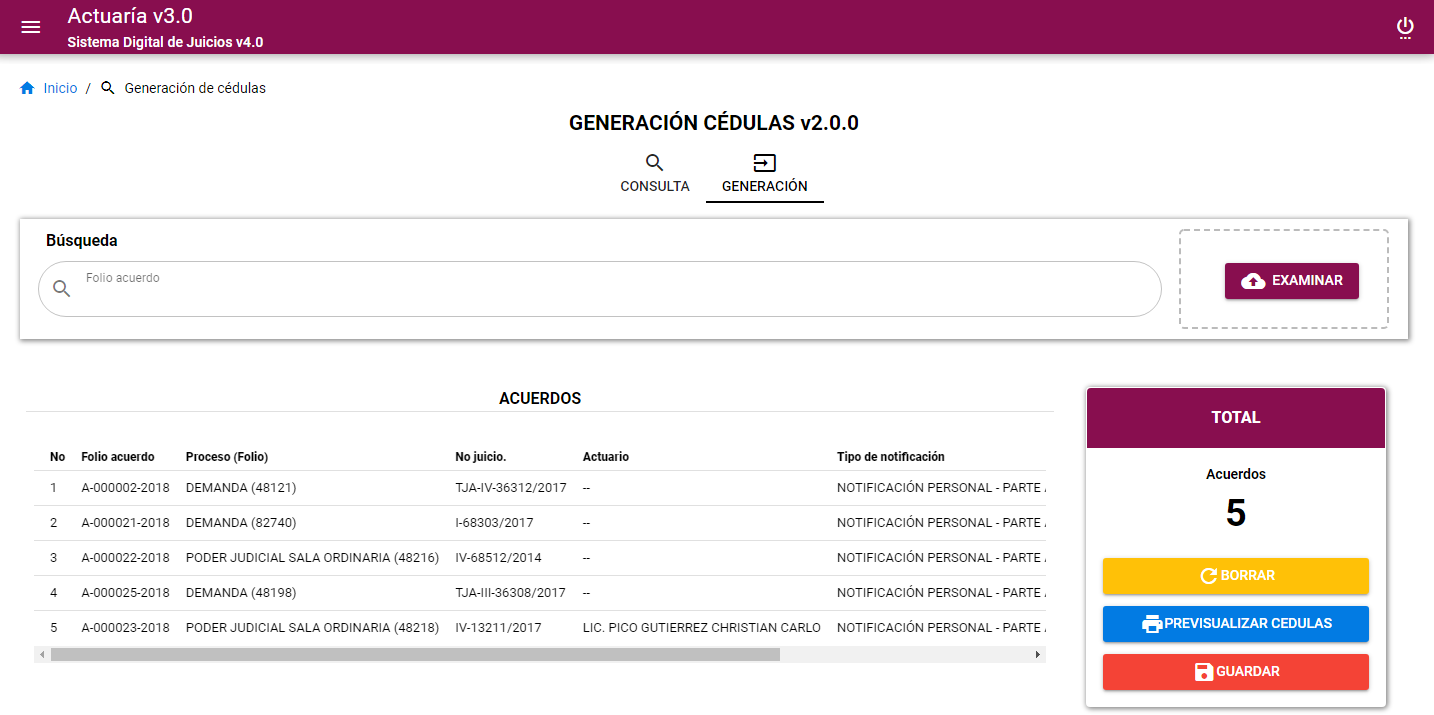
\includegraphics[width=0.90\columnwidth]{corregido.png}
\end{center}

Si lo deseamos podemos:\\
{{\bf
<<PRE VISUALIZAR CÉDULAS>> \\
<<BORRAR>> \\
<<GUARDAR>>
}}


\vspace{1cm}
2.{{\bf Borrar y volver a subir el archivo corregido}}\\
Daremos clic en el botón <<Borrar>>

\begin{center}
    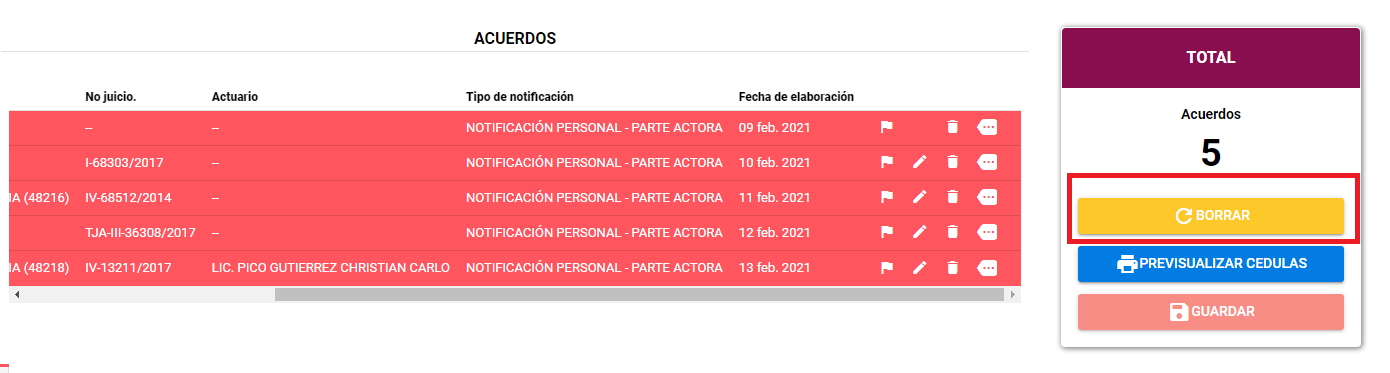
\includegraphics[width=0.90\columnwidth]{borraracuerdos.png}
\end{center}

Nos aparecerá una alerta:
\begin{center}
    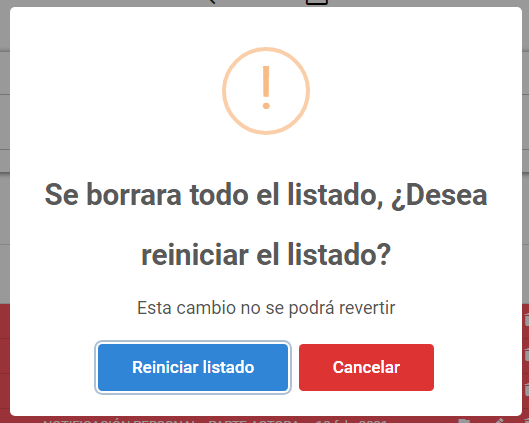
\includegraphics[width=0.50\columnwidth]{reiniciarlis.png}
\end{center}

Daremos clic en {{\bf<<Reiniciar listado>>}} en caso contrario daremos clic en <<Cancelar>>
nos aparecerá la pantalla sin nuestros acuerdos.

\begin{center}
    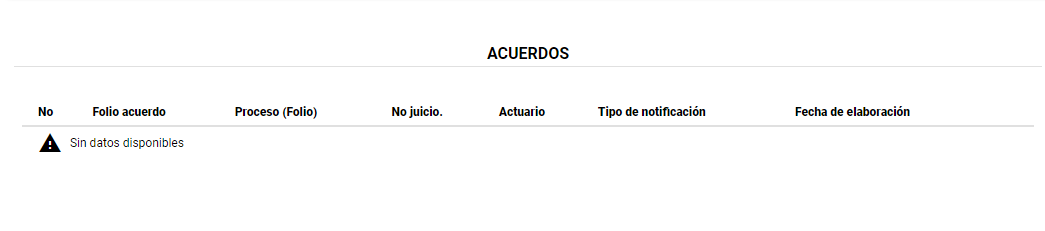
\includegraphics[width=0.90\columnwidth]{sindatos.png}
\end{center}

{\Huge{\color{myblue} \section{Lista de cédulas}\label{sec:14}}}
Para generar un listado de cédulas agregaremos los folios deseados, por cada folio 
agregado el sistema mostrara la siguiente ventana:

\begin{center}
    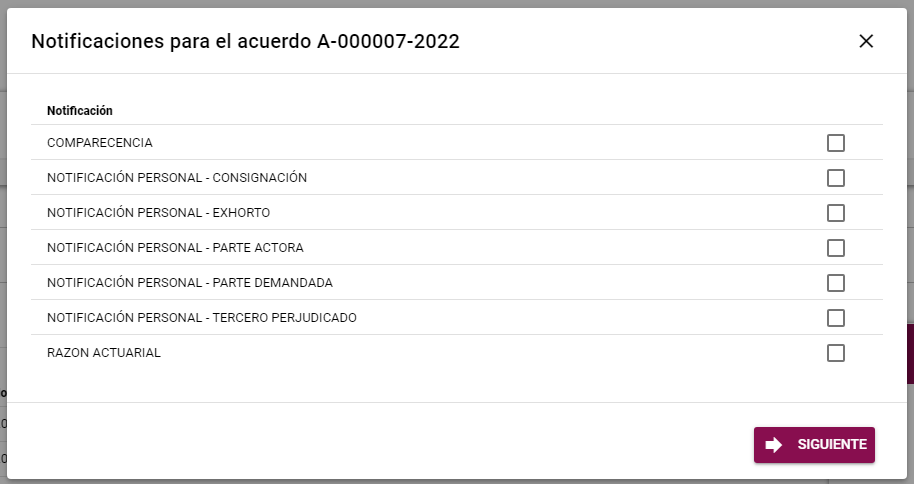
\includegraphics[width=0.80\columnwidth]{lista1.png}
\end{center}

Seleccionaremos las opciones deseadas y daremos clic en el botón {\bf{<<SIGUIENTE>>}}

Ahora llenaremos el formulario con los siguientes
datos:

\begin{center}
    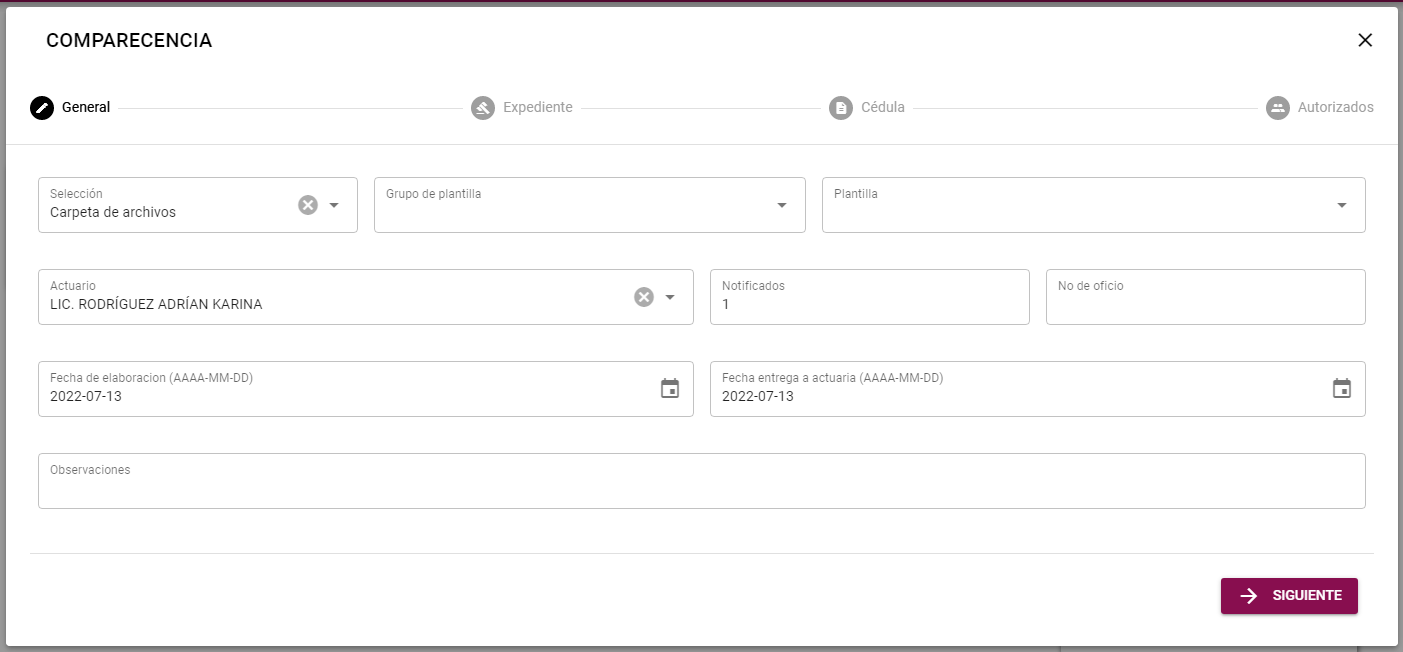
\includegraphics[width=0.90\columnwidth]{comparecencia.png}
\end{center}

\begin{itemize}
    \item Selección
    \item  Grupo de plantilla
    \item  Plantilla
    \item  Actuario
    \item  Notificados
    \item  No de oficio
    \item  Fecha entrega a actuaria
    \item  Fecha de elaboración
    \item Observaciones
\end{itemize}

En caso de no contar con una plantilla registrada en el sistema, se puede subir una plantilla
temporal.\\
Primero tienes que seleccionar:
{\bf{<<Subir archivo>>}}y dar clic en subir archivo.\\

\begin{center}
    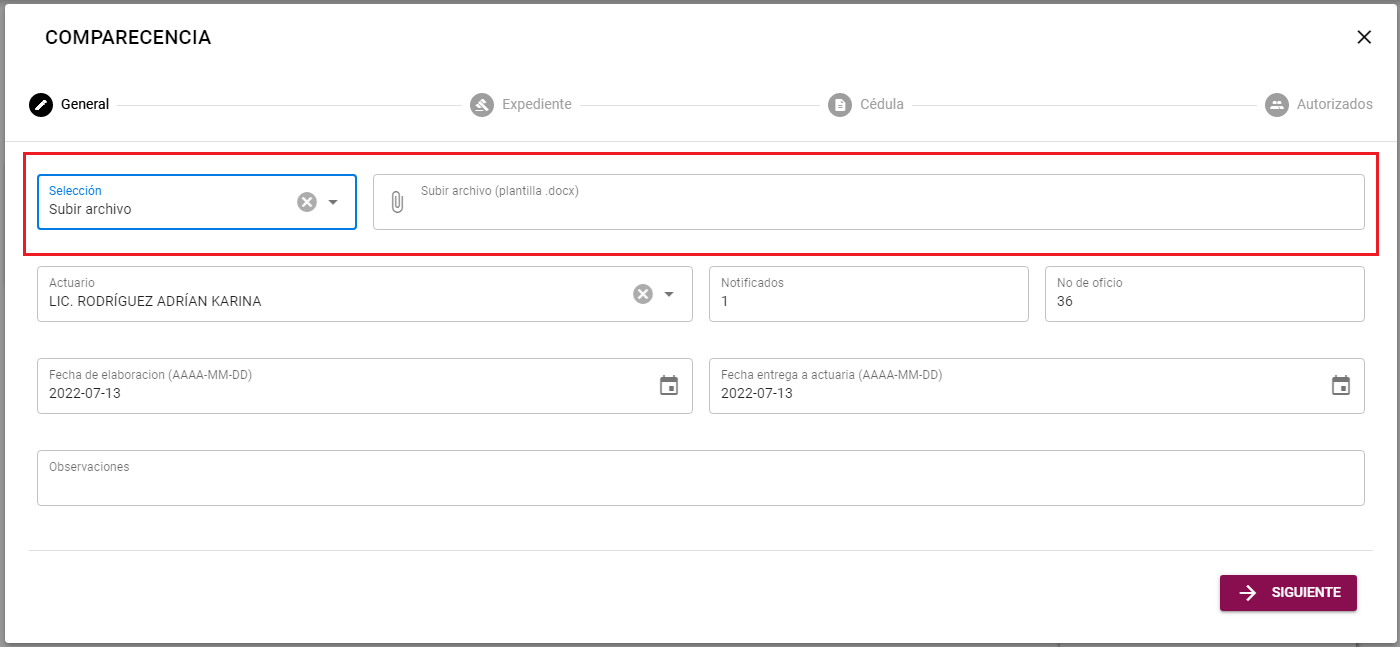
\includegraphics[width=0.90\columnwidth]{comparecencia3.png}
\end{center}

Automáticamente se abrirá una ventana donde seleccionaras tu plantilla desde tus documentos.

\begin{center}
    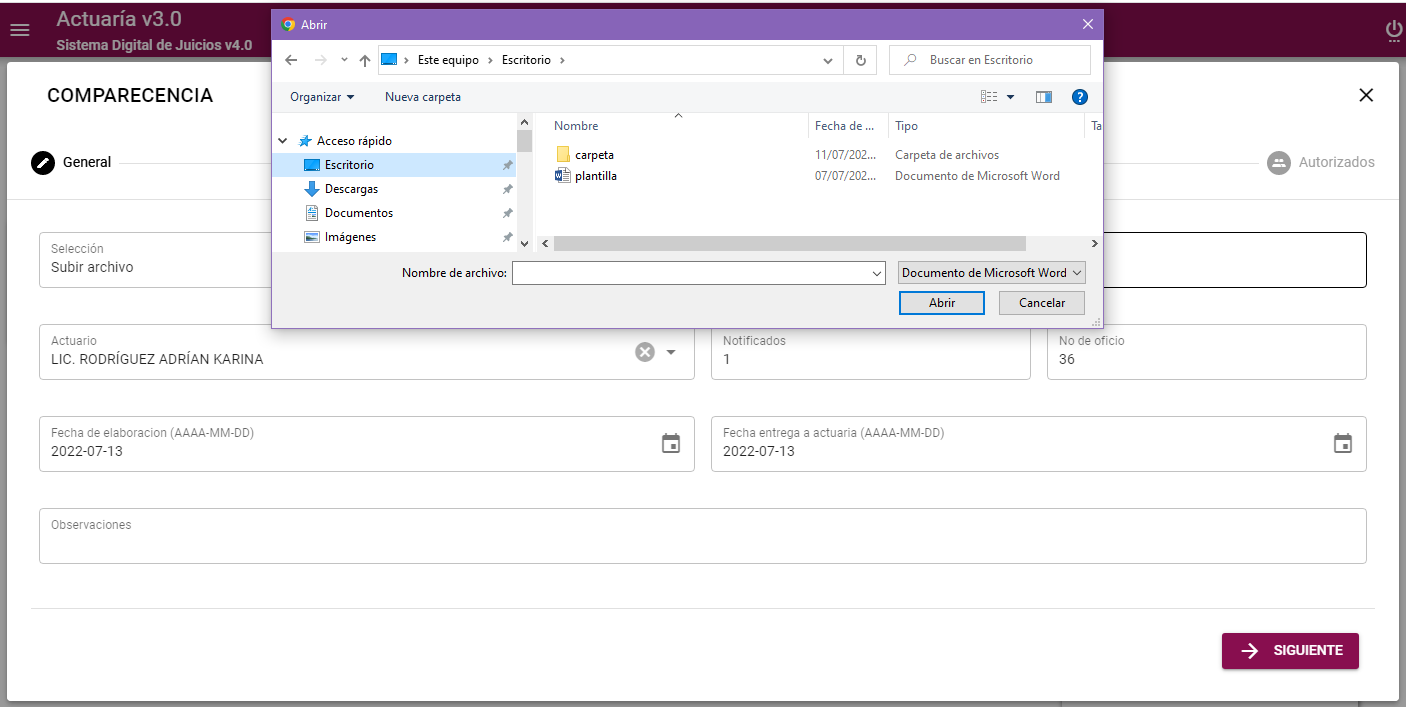
\includegraphics[width=0.90\columnwidth]{comparecencia4.png}
\end{center}

Después de ingresar los datos daremos clic en el botón.
{\bf{<<SIGUIENTE>>}}
Ahora ingresaremos los siguientes datos:

\begin{itemize}
    \item Teléfono
    \item Correo electrónico
    \item Domicilio para recibir notificaciones (*) 
\end{itemize}

\begin{center}
    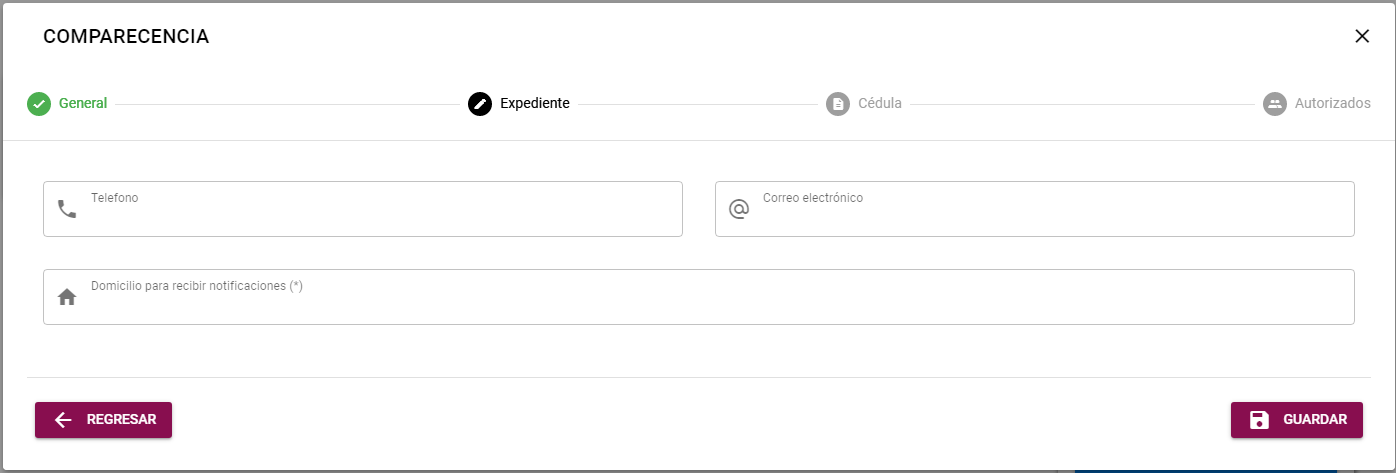
\includegraphics[width=0.90\columnwidth]{comparecencia2.png}
\end{center}

Daremos clic en {\bf{<<GUARDAR>>}}\\

Después llenaremos los siguientes datos:
\begin{center}
    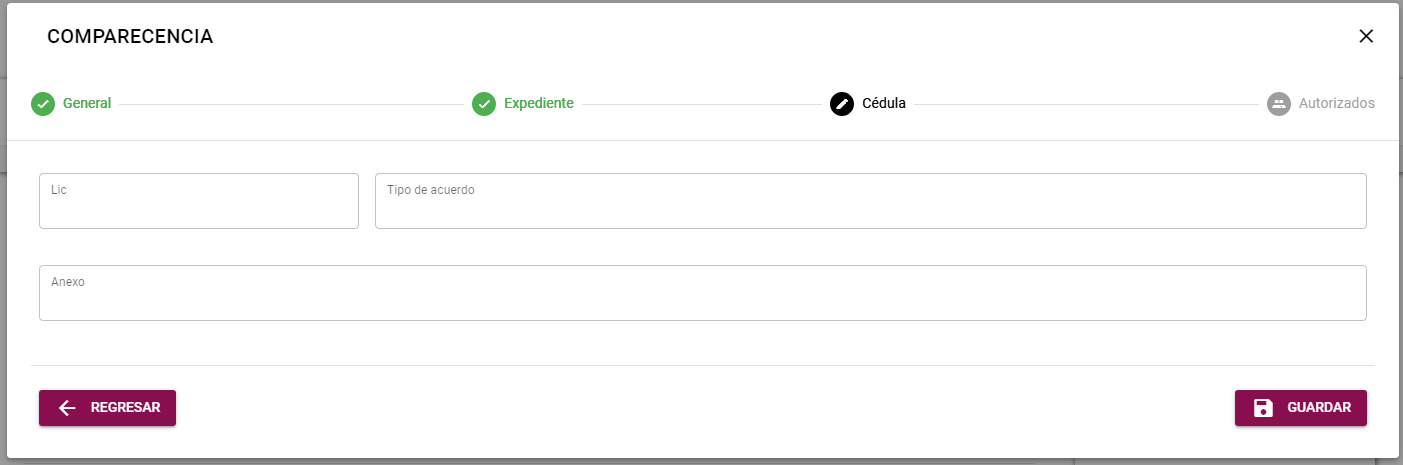
\includegraphics[width=0.90\columnwidth]{lista2.png}
\end{center}

Y daremos clic en {\bf{<<GUARDAR>>}}\\

Después podemos agregar representantes o dar clic en {\bf{<<GUARDAR>>}}
    
\begin{center}
    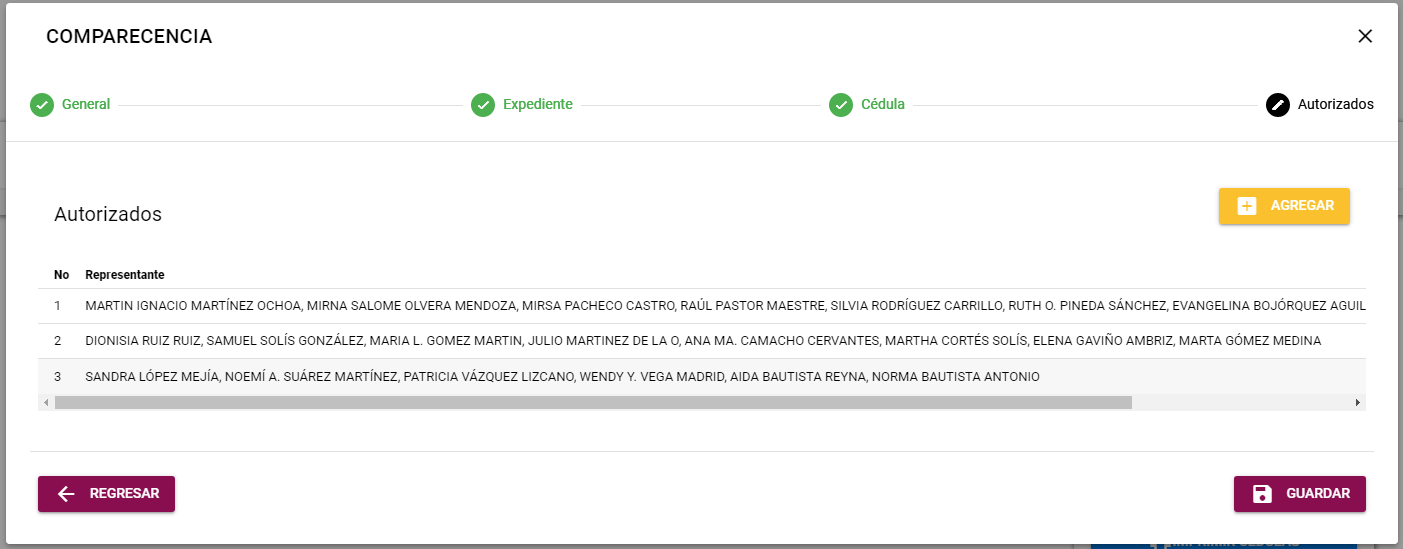
\includegraphics[width=0.90\columnwidth]{lista3.png}
\end{center}

Finalmente daremos clic en {\bf{<<GUARDAR>>}}.

{\Huge{\color{myblue} \section{Imprimir cédulas}\label{sec:15}}}

Podemos imprimir nuestras cédulas  dando clic en el botón {\bf{<<IMPRIMIR CÉDULAS>>}}

\begin{center}
    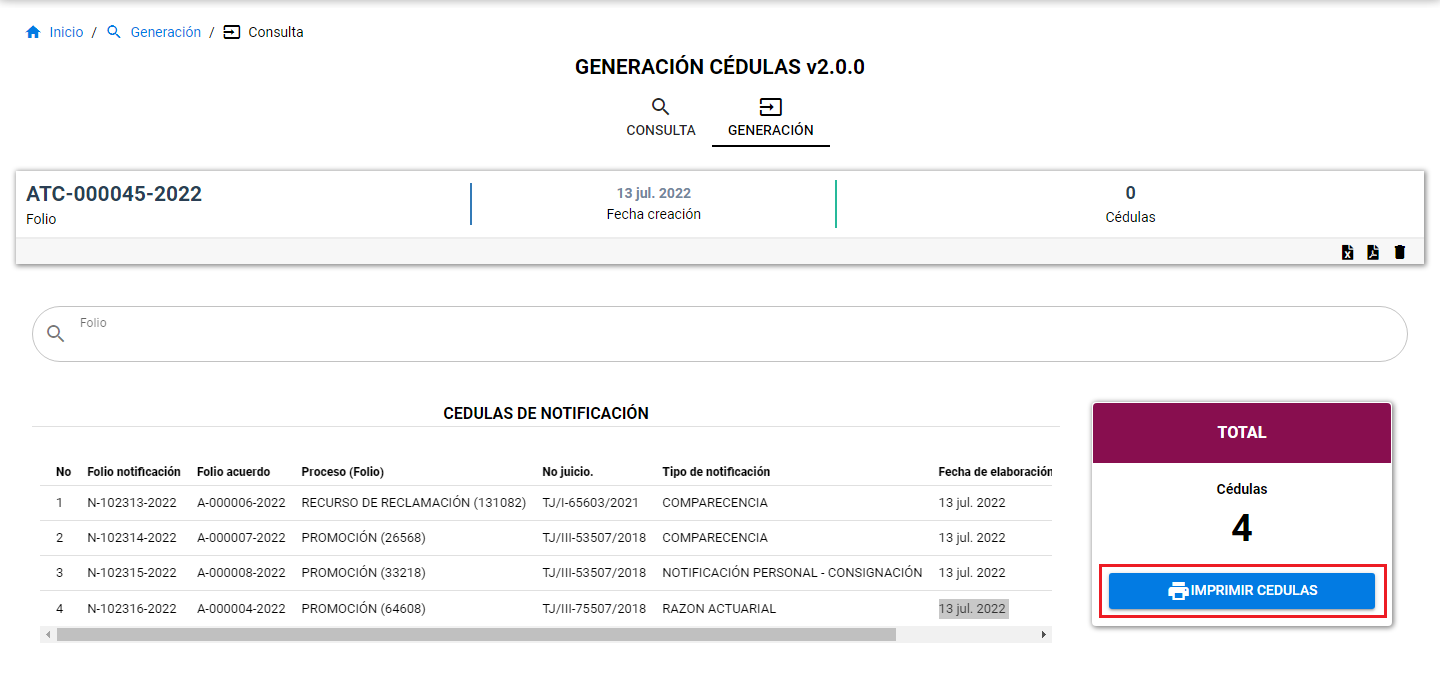
\includegraphics[width=0.88\columnwidth]{imprcedu.png}
\end{center}

Nos aparecerá una ventana donde podemos ver nuestras cédulas con su respectivo código de barras en la parte inferior derecha.

\begin{center}
    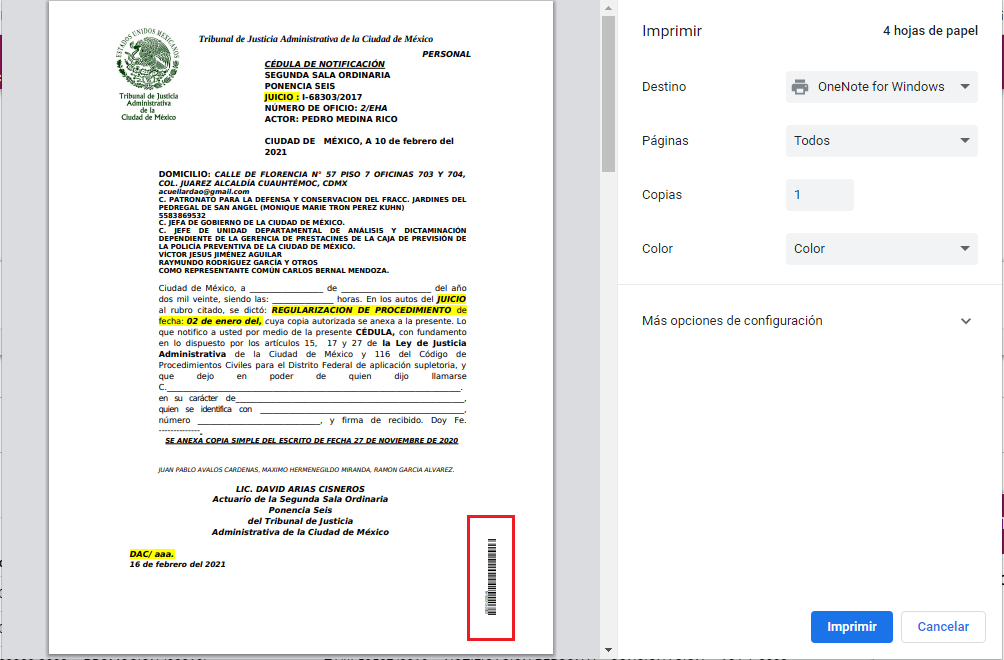
\includegraphics[width=0.90\columnwidth]{impcedula.png}
\end{center}

\newpage

{\Huge{\color{myblue} \section{Acciones}\label{sec:16}}}

Para cada notificación podemos realizar las siguientes acciones.

\begin{center}
    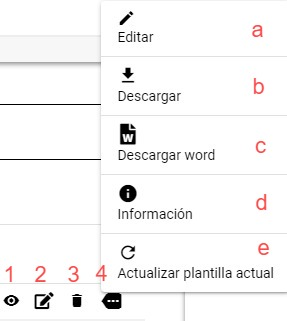
\includegraphics[width=.40\columnwidth]{masf.jpeg}
\end{center}


\begin{enumerate}[(1)]
    \item Visualizar cédula
    \item Editar
    \item Borrar
    \item Más
        \begin{enumerate}[(a)]
            \item Editar
            \item Descargar
            \item Descargar word
            \item Información
            \item Actualizar plantilla actual
        \end{enumerate}
\end{enumerate}


{\Huge{\color{myblue} \section{Visualizar cédula}\label{sec:17}}}
Para poder ver nuestra cédula basta con dar clic en el icono (1) y nos mostrará el archivo.
Ejemplo:

\begin{center}
    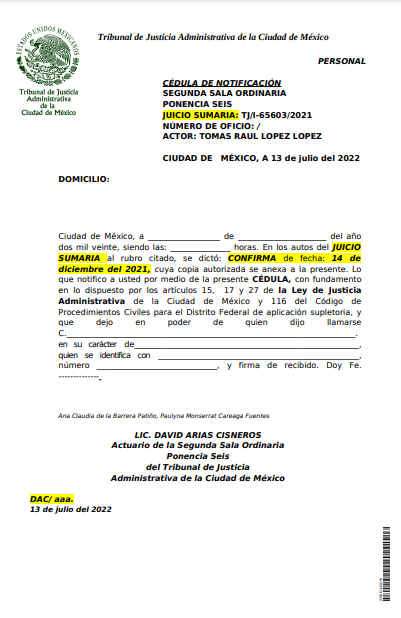
\includegraphics[width=0.77\columnwidth]{cedu.png}
\end{center}

{\Huge{\color{myblue} \section{Editar}\label{sec:18}}}
Para poder editar la cédula daremos clic en el icono (2) y nos mostrará la pantalla siguiente con las secciones de:

\begin{enumerate}[(1)]
    \item General
    \item Expediente
    \item Cédula
    \item Autorizados
    \item Actores
\end{enumerate}



\begin{center}
    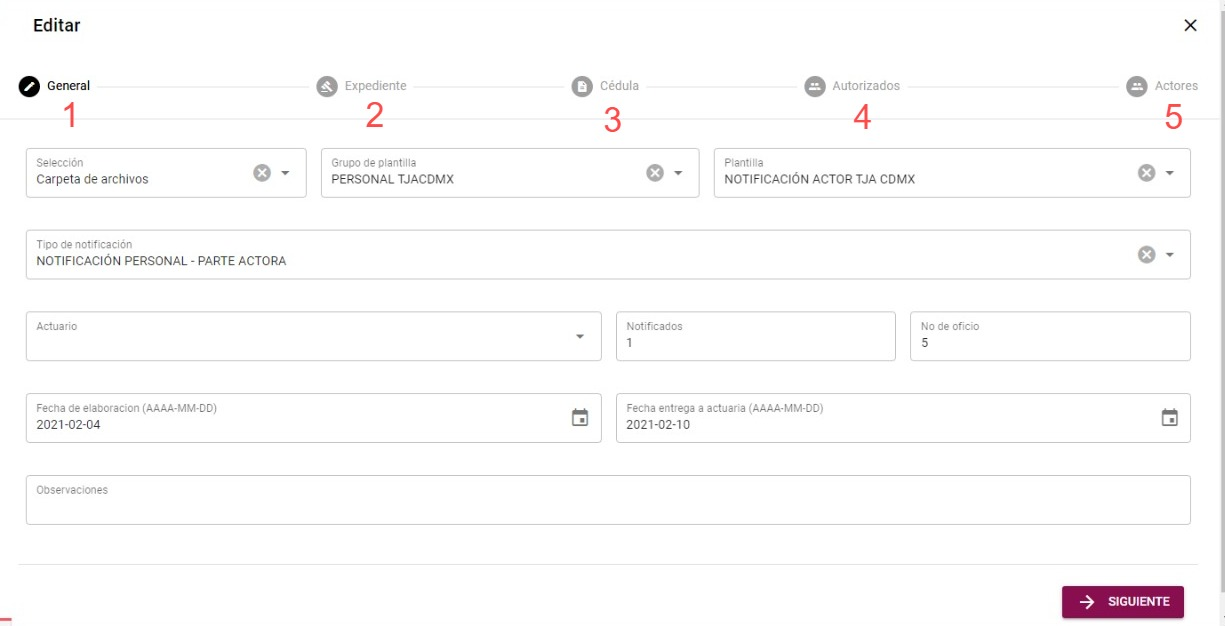
\includegraphics[width=0.90\columnwidth]{editar6.jpeg}
\end{center} En  General


Aquí ingresaremos los siguientes datos (1)  {\bf{
<<General>> :}}


\begin{enumerate}[(a)]
    \item Selección: Carpeta de archivos o subir archivo
    \item Grupo de plantilla
    \item Plantilla
    \item Tipo de notificación
    \item Actuario
    \item Notificados
    \item No oficio
    \item Fecha entrega a actuaria
    \item Fecha elaboración
    \item Observaciones
\end{enumerate}

Daremos clic en el botón  {{\bf<<SIGUIENTE>>}}
nos aparecerá la siguiente ventana:

\begin{center}
    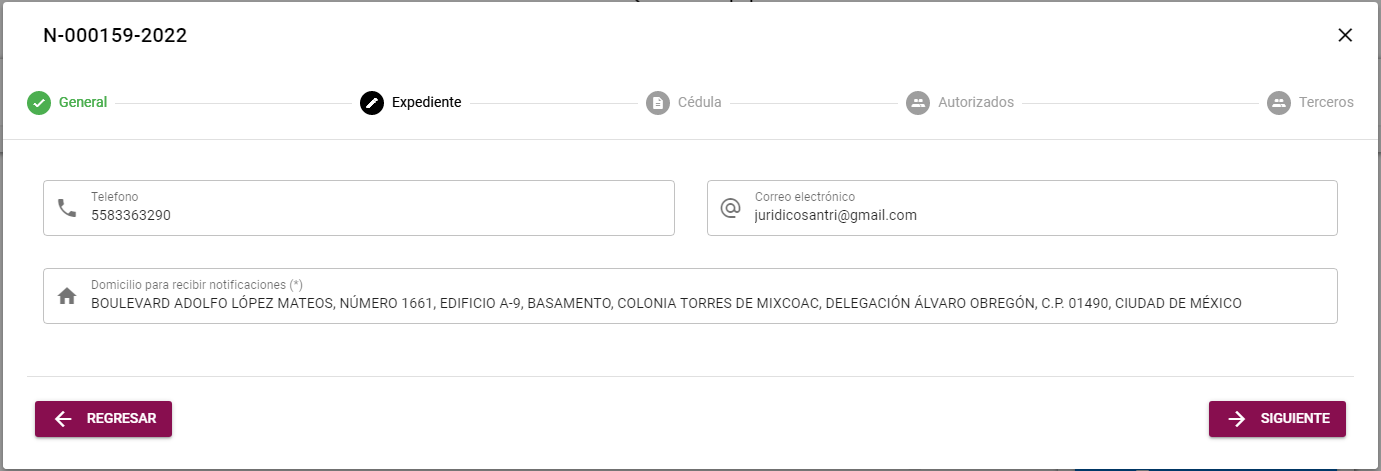
\includegraphics[width=.90\columnwidth]{editaracuerdo2.png}
\end{center}

Podemos revisar nuestros datos o corregir el deseado y
daremos clic en el botón  {{\bf<<SIGUIENTE>>}}
nos aparecerá la siguiente ventana:

\begin{center}
    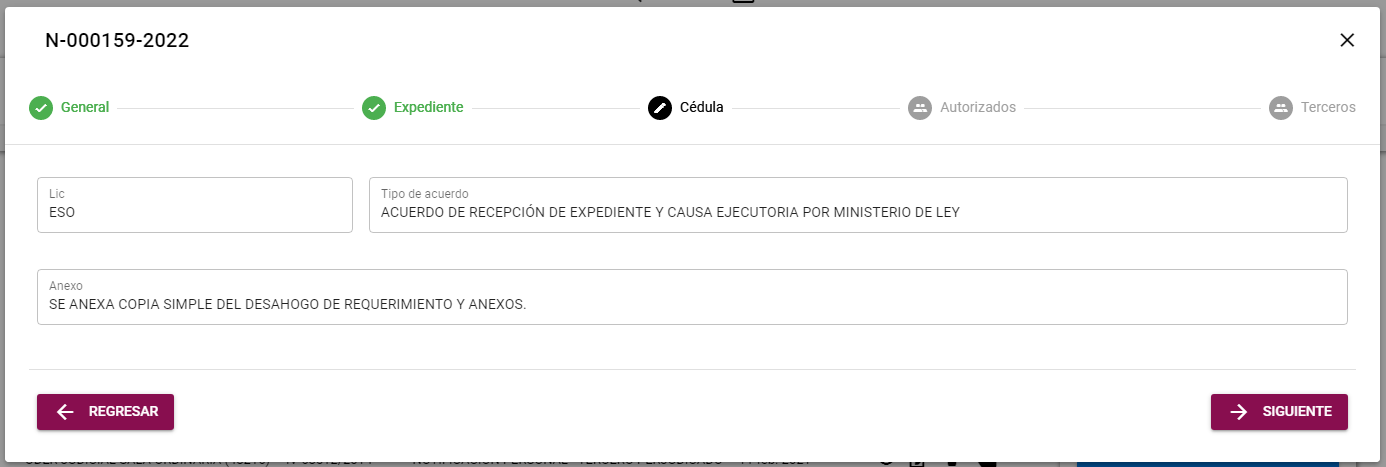
\includegraphics[width=.90\columnwidth]{editaracuerdo3.png}
\end{center}

De igual forma podemos revisar nuestros datos o corregir el deseado y
daremos clic en el botón  {{\bf<<SIGUIENTE>>}}
nos aparecerá la siguiente ventana:

\begin{center}
    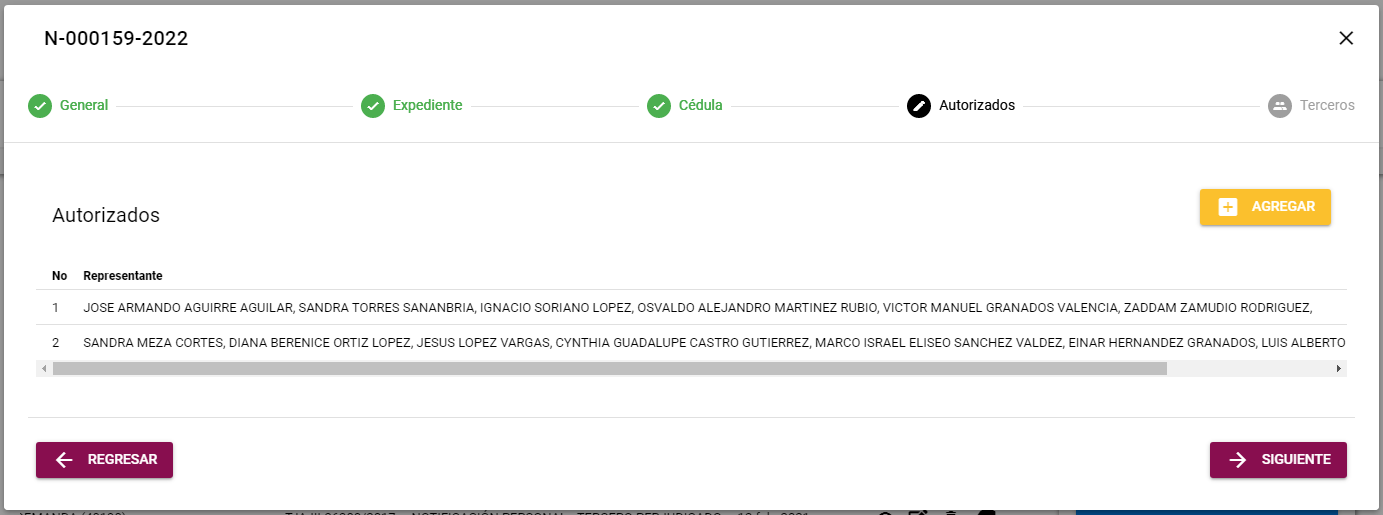
\includegraphics[width=.90\columnwidth]{editaracuerdo4.png}
\end{center}

daremos clic en el botón  {{\bf<<SIGUIENTE>>}}
nos aparecerá la siguiente ventana:

\begin{center}
    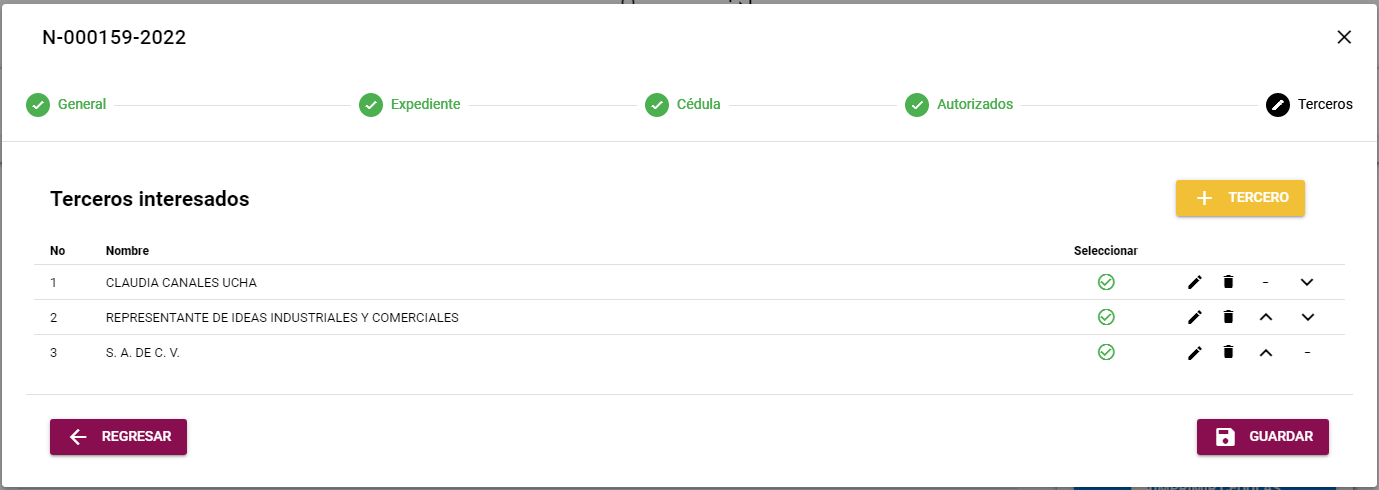
\includegraphics[width=0.90\columnwidth]{editaracuerdo5.png}
\end{center}

Daremos clic en el botón {\bf{<<GUARDAR>>}} si los datos de nuestros acuerdos son correctos nos aparecerá el siguiente mensaje:

\begin{center}
    
\includegraphics[width=0.30\columnwidth]{cedulaguardada.png}
\end{center}

Seguido de este mensaje.
\begin{center}
    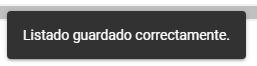
\includegraphics[width=0.33\columnwidth]{listadoguardado.png}
\end{center}

Ahora ya podemos visualizar nuestros acuerdos corregidos.
\begin{center}
    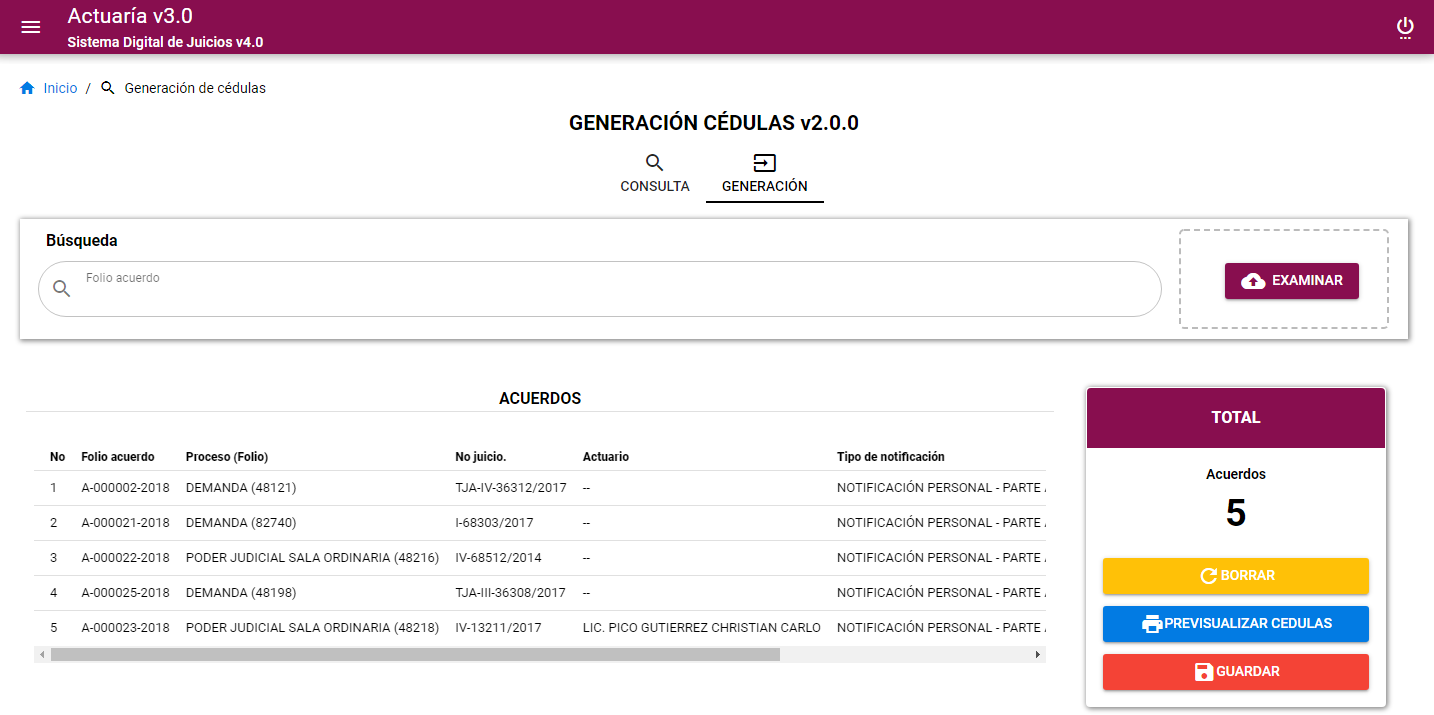
\includegraphics[width=0.90\columnwidth]{corregido.png}
\end{center}

Si lo deseamos podemos:\\
{{\bf
<<PREVISUALIZAR CÉDULAS>> \\
<<BORRAR>> \\
<<GUARDAR>>
}}


En caso de no contar con una plantilla registrada en el sistema, se puede subir una plantilla
temporal.\\
Primero tienes que seleccionar:
Subir archivo.\\
y dar clic en subir archivo para que abra la ventana para seleccionar archivo.

\begin{center}
    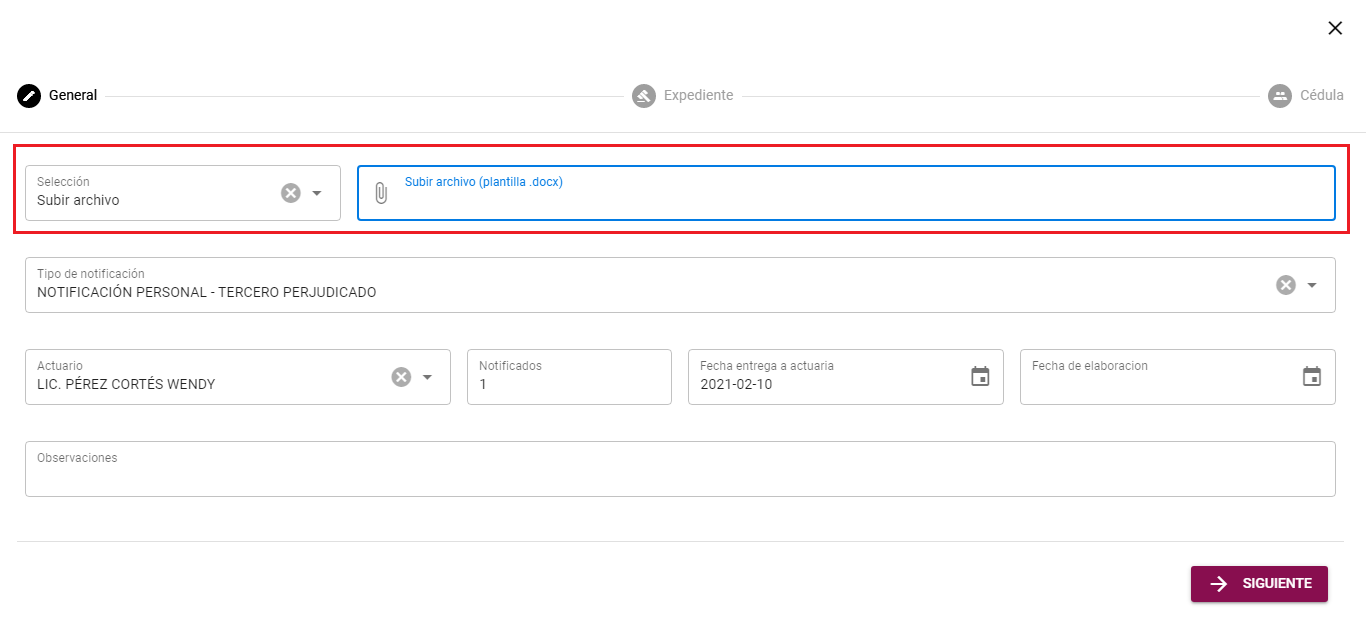
\includegraphics[width=.90\columnwidth]{subira.png}
\end{center}

Después de ingresar los datos daremos clic en {\bf{
<<SIGUIENTE>>}}

\begin{center}
    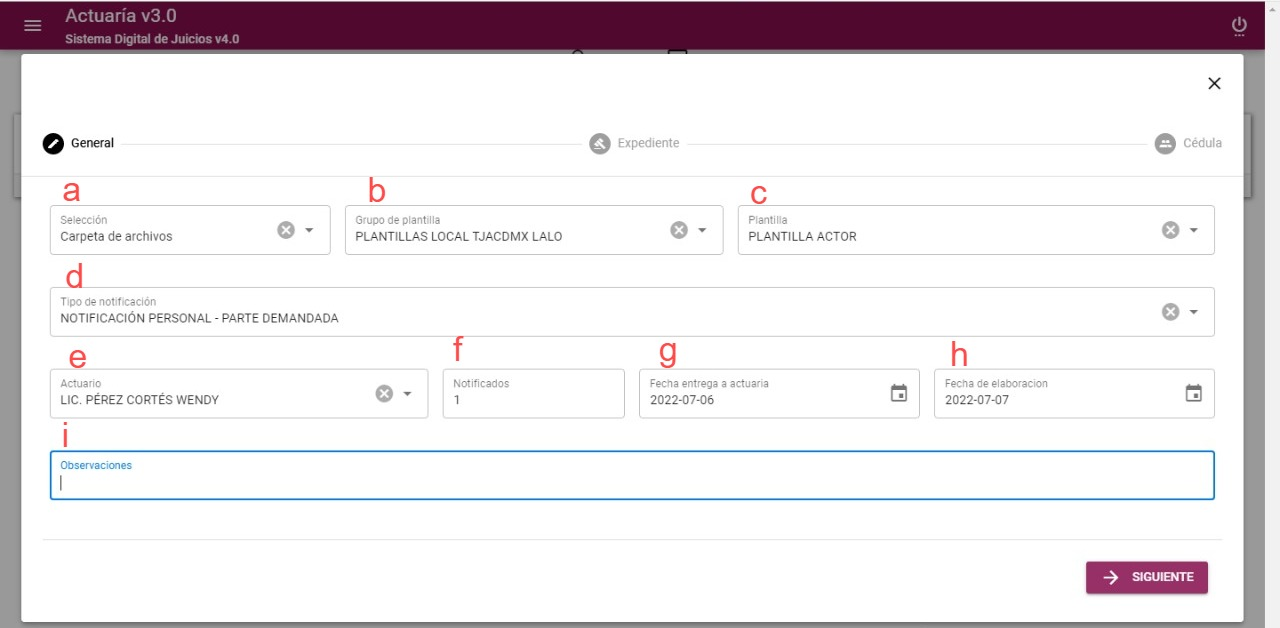
\includegraphics[width=.90\columnwidth]{op2.jpeg}
\end{center}

Ahora ingresaremos: {\bf{Domicilio para recibir notificaciones.}}
\begin{center}
    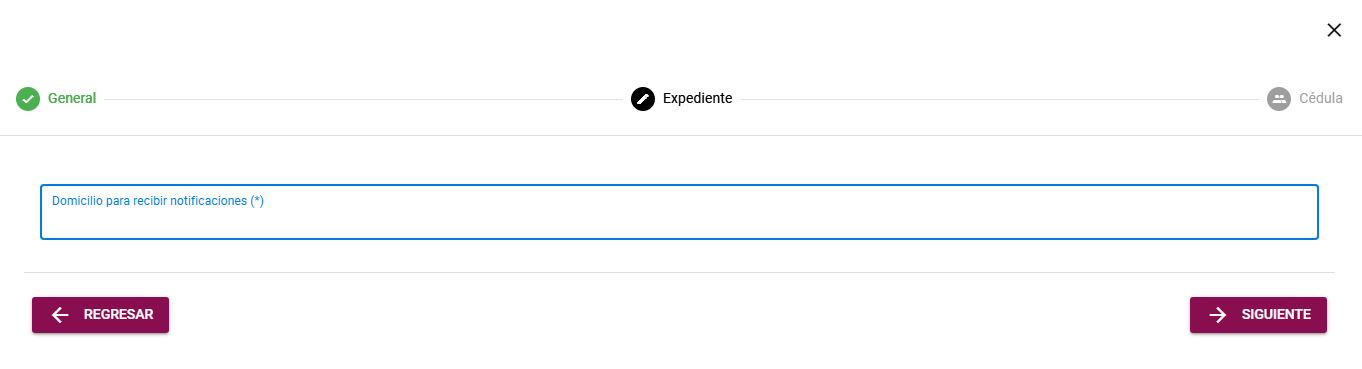
\includegraphics[width=.90\columnwidth]{op3.png}
\end{center}

Daremos clic en {\bf{<<SIGUIENTE>>}}
Podemos agregar {\bf{ <<Actor, Autoridad>>}} para  agregar Actor(es)
solo deberá de dar clic en el botón  {\bf{ «+ ACTOR»}}, e ingresar la siguiente información:

\begin{multicols}{2}
\begin{itemize}
    \item Tipo de persona.
    \item Nombre.
    \item Apellido paterno.
    \item Apellido materno.
    \item Genero.
    \item Teléfono.
    \item Correo.
    \item Delegación.
    \item Domicilio.
\end{itemize}
\end{multicols}


\begin{center}
    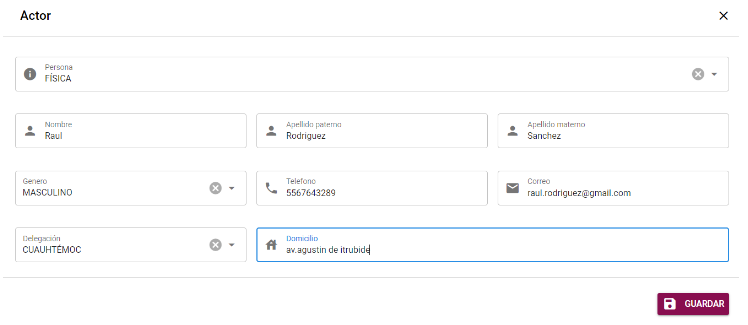
\includegraphics[width=0.90\columnwidth]{actor.png}
\end{center}

A continuación, deberá dar clic en el botón {\bf{«GUARDAR»}}, mostrara la lista de los actores registrados.

Para borrar un actor solo debes de dar clic el icono borrar       

\includegraphics[width=0.05\columnwidth]{iconob.png}\\

Nos mostrara un mensaje de confirmación,
da clic en el botón {\bf{«BORRAR»}} si está seguro.\\
El actor se quitará automáticamente de la lista de
actores, en caso de no estar seguro de borrar al actor solo debe de dar clic {\bf{«CANCELAR».}}\\
\vspace{1cm}
Podemos observar las cédulas de notificación registradas, debe de dar clic en el botón {\bf{«GUARDAR»}} para que
se guarde correctamente el listado, en caso de borrar todo el listado solo debe de dar clic el botón
{\bf{«BORRAR»}}, para que se reinicie el listado.\\
\newpage
En el caso de {\bf{''Autoridades''}} aquí podemos:

\begin{center}
    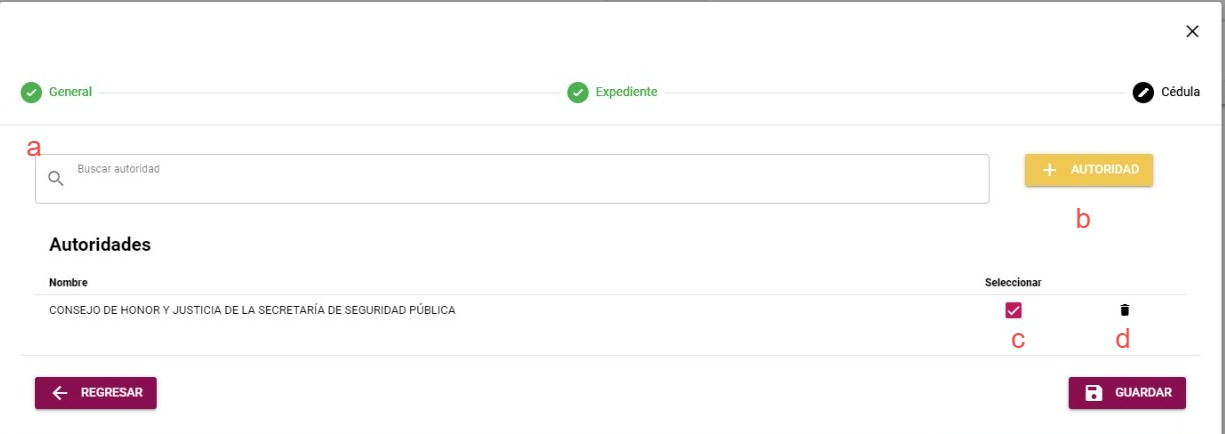
\includegraphics[width=0.90\columnwidth]{op4.jpeg}
\end{center}

\begin{item}
    \item (a) Buscar autoridad
    \item (b) Agregar autoridad
    \item (c) Seleccionar autoridad
    \item (d) Eliminar autoridad
\end{item}


(a) {\bf{<<Buscar autoridad>>}} basta con escribir dentro de nuestro buscador y en
{\bf{
<<Autoridades>>}}
nos aparecerá.

(b) Añadir una autoridad  daremos clic en el botón 
\includegraphics[width=0.15\columnwidth]{botautoridad.png} y nos aparecerá la siguiente pantalla:
\begin{center}
    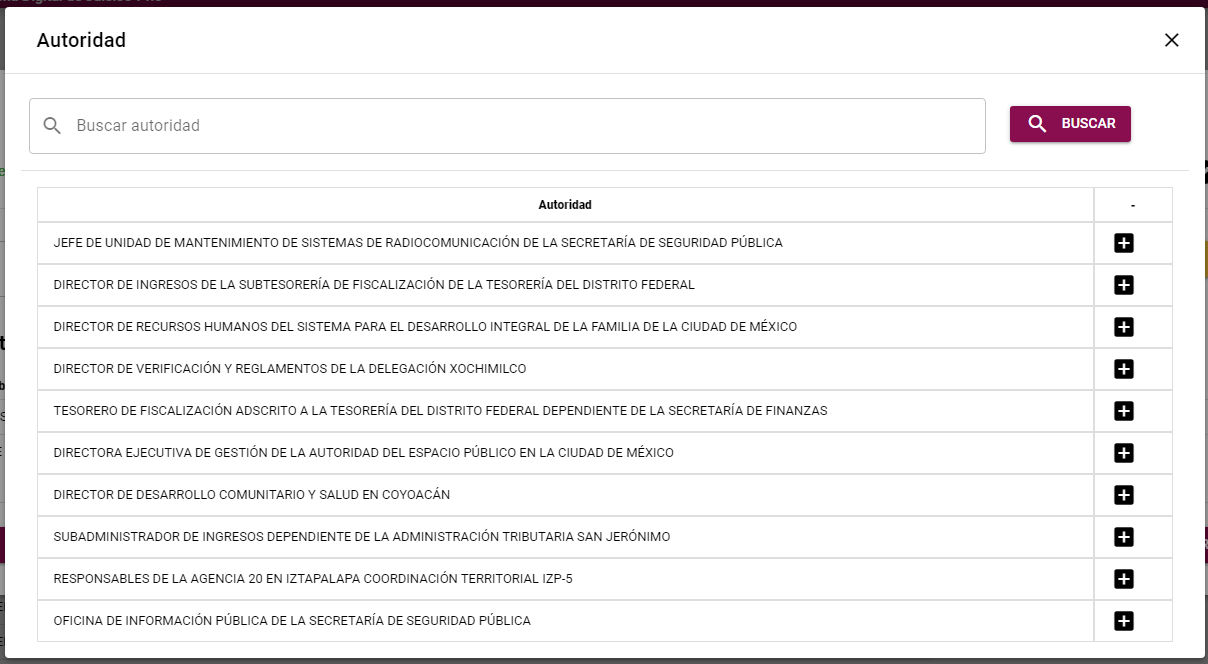
\includegraphics[width=0.90\columnwidth]{auto1.png}
\end{center}

Podemos dar clic en el botón + para agregarla o buscarla y dar clic en el botón {\bf{<<buscar>>}}
para después dar clic en el botón + y agregarla y nos aparecerá en Autoridades

\begin{center}
    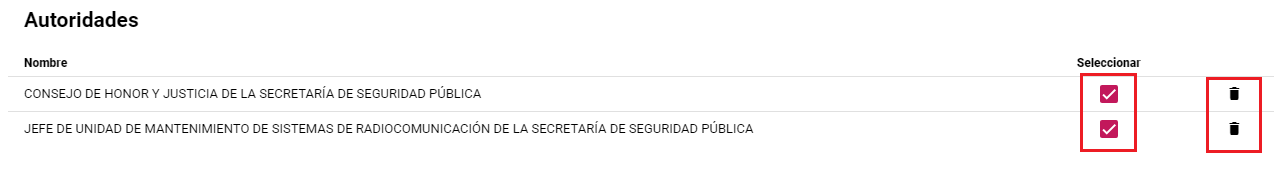
\includegraphics[width=0.90\columnwidth]{auto2.png}
\end{center}

Daremos clic en (c) {\bf{<<seleccionar>> }}
o bien (d) Eliminar  si lo requerimos.\\
Después daremos clic en el botón  \includegraphics[width=.15\columnwidth]{GUARDAR.png}

{\Huge{\color{myblue} \section{Borrar}\label{sec:20}}}
Podemos borrar la notificación dando clic en el icono (3).

{\Huge{\color{myblue} \section{Más}\label{sec:21}}}
La opción Más (4) nos ofrece las siguientes opciones:

\begin{center}
    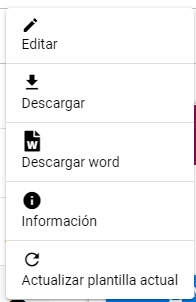
\includegraphics[width=0.20\columnwidth]{mas_cedulas.png}
\end{center}

{\bf{ <<Editar notificación>>}} Nos permite editar la notificación
\begin{center}
    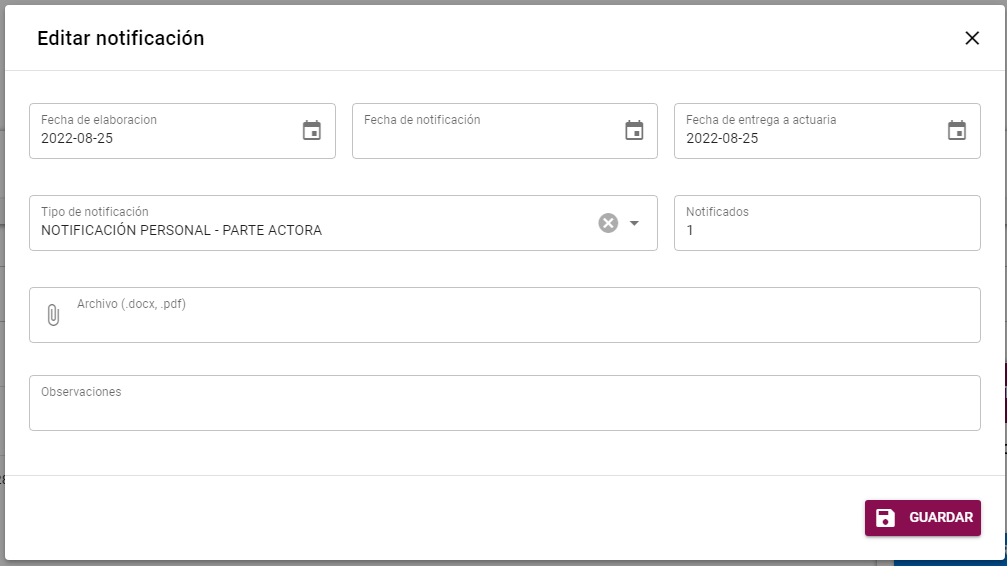
\includegraphics[width=0.70\columnwidth]{edi_noti.png}
\end{center}

{\bf{ <<Descarga>>}}
Esta opción nos permite descargar a nuestro equipo el archivo en formato pdf.\\

{\bf{ <<Descargar en word>>}}
Esta opción nos permite descargar a nuestro equipo el archivo en formato word.\\
{\bf{ <<Información>>}}
Esta opción nos permite ver detalles de la cédula.\\

\begin{center}
    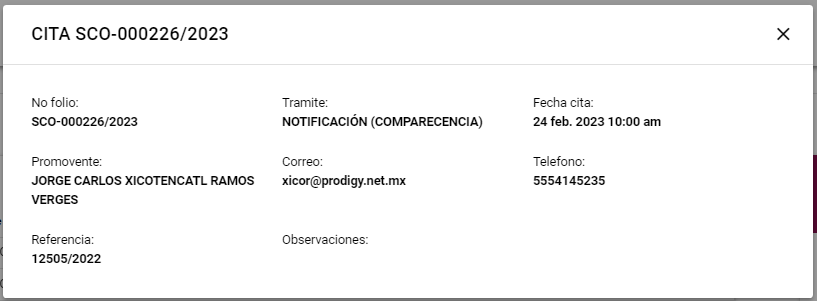
\includegraphics[width=0.70\columnwidth]{inf.png}
\end{center}

{\bf{<<Actualizar plantilla>>}} Nos permite actualizar la plantilla a la versión más reciente, daremos clic en  {\bf{ <<Actualizar>>}}
\begin{center}
    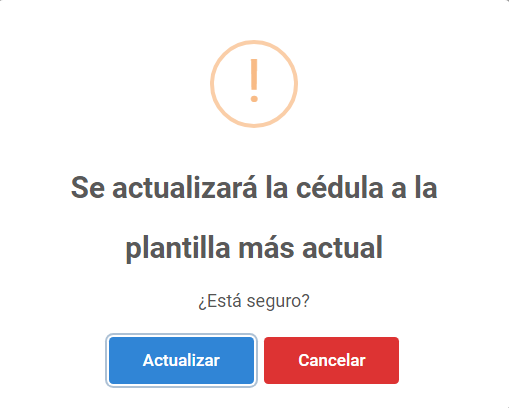
\includegraphics[width=0.40\columnwidth]{alet.png}
\end{center}

{\Huge{\color{myblue} \section{Borrar listado}\label{sec:22}}}
Para borrar el listado daremos clic en el botón     

\includegraphics[width=0.15\columnwidth]{borrarlist.png} y nos aparecerá la siguiente pantalla

\begin{center}
    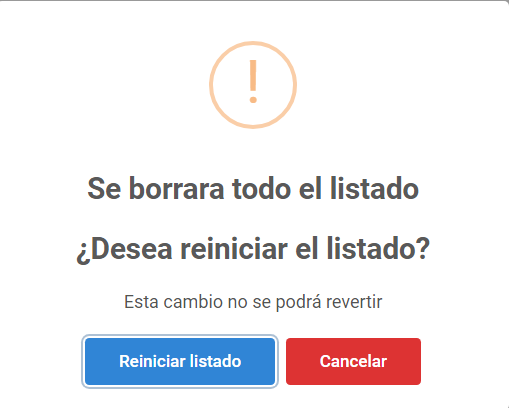
\includegraphics[width=0.50\columnwidth]{blist.png}
\end{center} 

daremos clic en Reiniciar listado.

{\Huge{\color{myblue} \section{Imprimir listado}\label{sec:23}}}

Para imprimir un listado tenemos que dar clic en el botón.


\includegraphics[width=0.15\columnwidth]{imprilist.png} nos 
abrirá una nueva pagina donde daremos clic en el botón imprimir.


\newpage
\begin{table}[t]
\begin{center}
\begin{tabular}{| c | c | c | c | }
\hline

\multicolumn{4}{ |c| }{\cellcolor[gray]{0.9}CONTROL DE VERSIONES} \\ \hline
Versión &               Elaborado por:          & Fecha de última modificación          & Motivo \\ \hline
1.0.1   & Esthefania Vidal Solares        &      12/octubre/2022
&Creación \\ \hline
1.0.2   & Esthefania Vidal Solares        &     27/febrero/2023
&Actualización \\ \hline
\hline
\end{tabular}
\caption{Control de Versiones}
\label{tab:versiones}
\end{center}
\end{table}

\end{quote}

\end{document}